%%%%%%%% ICML 2025 EXAMPLE LATEX SUBMISSION FILE %%%%%%%%%%%%%%%%%

\documentclass{article}

% Recommended, but optional, packages for figures and better typesetting:
\usepackage{microtype}
\usepackage{graphicx}
\usepackage{subcaption}

%\usepackage{subfigure}
\usepackage{booktabs} % for professional tables

% hyperref makes hyperlinks in the resulting PDF.
% If your build breaks (sometimes temporarily if a hyperlink spans a page)
% please comment out the following usepackage line and replace
% \usepackage{icml2025} with \usepackage[nohyperref]{icml2025} above.
\usepackage{hyperref}


% Attempt to make hyperref and algorithmic work together better:
\newcommand{\theHalgorithm}{\arabic{algorithm}}

% Use the following line for the initial blind version submitted for review:
 %\usepackage{icml2025}

% If accepted, instead use the following line for the camera-ready submission:
\usepackage[accepted]{icml2025}

% For theorems and such
\usepackage{amsmath}
\usepackage{amssymb}
\usepackage{mathtools}
\usepackage{amsthm}
\usepackage{color}
\usepackage{xspace}
%\usepackage{algcompatible}
\usepackage{algorithm,algorithmic}
\usepackage{threeparttable}
\usepackage{breakurl}

\def\UrlBreaks{\do\/\do-}
%\renewcommand{\algorithmicrequire}{\textbf{Input:}}
%\renewcommand{\algorithmicensure}{\textbf{Output:}}


% if you use cleveref..
\usepackage[capitalize,noabbrev]{cleveref}
\usepackage{enumitem,amssymb}
\newlist{todolist}{itemize}{2}
\setlist[todolist]{label=$\square$}
%%%%%%%%%%%%%%%%%%%%%%%%%%%%%%%%
% THEOREMS
%%%%%%%%%%%%%%%%%%%%%%%%%%%%%%%%
\theoremstyle{plain}
\newtheorem{theorem}{Theorem}[section]
\newtheorem{proposition}[theorem]{Proposition}
\newtheorem{lemma}[theorem]{Lemma}
\newtheorem{corollary}[theorem]{Corollary}
\theoremstyle{definition}
\newtheorem{definition}[theorem]{Definition}
\newtheorem{assumption}[theorem]{Assumption}
\theoremstyle{remark}
\newtheorem{remark}[theorem]{Remark}


% Todonotes is useful during development; simply uncomment the next line
%    and comment out the line below the next line to turn off comments
%\usepackage[disable,textsize=tiny]{todonotes}
\usepackage[textsize=tiny]{todonotes}

\newif\ifcomm
\commtrue
%\commfalse


\newcommand{\lc}[1]{{\color{magenta} \ifcomm \texttt{} Lydia: #1 \fi}}
\newcommand{\NB}[1]{{\color{blue} \ifcomm \texttt{} Nick: #1 \fi}}
\newcommand{\onote}[1]{{\color{teal} \ifcomm \texttt{} Ozzy: #1 \fi}}

\newcommand{\sys}{\texttt{SkipPipe}\xspace}
\newcommand{\cc}[1]{\texttt{CC#1}\xspace}
\newcommand{\tc}[1]{\texttt{TC#1}\xspace}
\newcommand{\hr}[1]{\textit{HR#1}\xspace}
%\newcommand{\type0}{\texttt{CC1}\xspace}
%\newcommand{\typeI}{\texttt{CC2}\xspace}
%\newcommand{\typeII}{\texttt{TC1}\xspace}
%\newcommand{\typeIII}{\texttt{TC2}\xspace}


\usepackage{soul}
% The \icmltitle you define below is probably too long as a header.
% Therefore, a short form for the running title is supplied here:
\icmltitlerunning{\sys:  Partial Pipeline Parallelism}

 
\begin{document}

\twocolumn[
\icmltitle{\sys: Partial and Reordered Pipelining Framework for Training LLMs in Heterogeneous Networks}



% It is OKAY to include author information, even for blind
% submissions: the style file will automatically remove it for you
% unless you've provided the [accepted] option to the icml2025
% package.

% List of affiliations: The first argument should be a (short)
% identifier you will use later to specify author affiliations
% Academic affiliations should list Department, University, City, Region, Country
% Industry affiliations should list Company, City, Region, Country

% You can specify symbols, otherwise they are numbered in order.
% Ideally, you should not use this facility. Affiliations will be numbered
% in order of appearance and this is the preferred way.
\icmlsetsymbol{equal}{*}

\begin{icmlauthorlist}
\icmlauthor{Nikolay Blagoev}{wt}
\icmlauthor{Lydia Yiyu Chen}{un}
\icmlauthor{O\u{g}uzhan Ersoy}{ga}
\end{icmlauthorlist}

\icmlaffiliation{wt}{Worker Thread}
\icmlaffiliation{un}{University of Neuchatel \& TU Delft}
\icmlaffiliation{ga}{Gensyn}


\icmlcorrespondingauthor{Nikolay Blagoev}{workerthreadllc@gmail.com}
% \icmlcorrespondingauthor{Firstname2 Lastname2}{first2.last2@www.uk}

% You may provide any keywords that you
% find helpful for describing your paper; these are used to populate
% the "keywords" metadata in the PDF but will not be shown in the document
\icmlkeywords{LLM, Distributed Training, Scheduling}

\vskip 0.3in
]

% this must go after the closing bracket ] following \twocolumn[ ...

% This command actually creates the footnote in the first column
% listing the affiliations and the copyright notice.
% The command takes one argument, which is text to display at the start of the footnote.
% The \icmlEqualContribution command is standard text for equal contribution.
% Remove it (just {}) if you do not need this facility.

\printAffiliationsAndNotice{}  % leave blank if no need to mention equal contribution
%\printAffiliationsAndNotice{\icmlEqualContribution} % otherwise use the standard text.

\begin{abstract}
 
Data and pipeline parallelism are ubiquitous for training of Large Language Models (LLM) on distributed nodes. Driven by the need for cost-effective training, recent work explores efficient communication arrangement for end to end training. Motivated by LLM's resistance to layer skipping and layer reordering, in this paper, we explore stage (several consecutive layers) skipping in pipeline training, and challenge the conventional practice of sequential pipeline execution. We derive convergence and throughput constraints (guidelines) for pipelining with skipping and swapping pipeline stages.
Based on these constraints, we propose \sys, the first partial pipeline framework to reduce the end-to-end training time for LLMs while preserving the convergence. The core of \sys is a path scheduling algorithm that optimizes the paths for individual microbatches and reduces 
idle time (due to microbatch collisions) on the distributed nodes, complying with the given stage skipping ratio.  We extensively evaluate \sys on LLaMa models from 500M to 8B parameters on up to 20 nodes. Our results show that \sys reduces training iteration time by up to 55\% compared to full pipeline.
 Our partial pipeline training also improves resistance to layer omission during inference, experiencing a drop in perplexity of only 7\% when running only half the model. Our code is available at \url{https://github.com/gensyn-ai/skippipe}.

\end{abstract}


\section{Introduction}
\label{sec:introduction}
The business processes of organizations are experiencing ever-increasing complexity due to the large amount of data, high number of users, and high-tech devices involved \cite{martin2021pmopportunitieschallenges, beerepoot2023biggestbpmproblems}. This complexity may cause business processes to deviate from normal control flow due to unforeseen and disruptive anomalies \cite{adams2023proceddsriftdetection}. These control-flow anomalies manifest as unknown, skipped, and wrongly-ordered activities in the traces of event logs monitored from the execution of business processes \cite{ko2023adsystematicreview}. For the sake of clarity, let us consider an illustrative example of such anomalies. Figure \ref{FP_ANOMALIES} shows a so-called event log footprint, which captures the control flow relations of four activities of a hypothetical event log. In particular, this footprint captures the control-flow relations between activities \texttt{a}, \texttt{b}, \texttt{c} and \texttt{d}. These are the causal ($\rightarrow$) relation, concurrent ($\parallel$) relation, and other ($\#$) relations such as exclusivity or non-local dependency \cite{aalst2022pmhandbook}. In addition, on the right are six traces, of which five exhibit skipped, wrongly-ordered and unknown control-flow anomalies. For example, $\langle$\texttt{a b d}$\rangle$ has a skipped activity, which is \texttt{c}. Because of this skipped activity, the control-flow relation \texttt{b}$\,\#\,$\texttt{d} is violated, since \texttt{d} directly follows \texttt{b} in the anomalous trace.
\begin{figure}[!t]
\centering
\includegraphics[width=0.9\columnwidth]{images/FP_ANOMALIES.png}
\caption{An example event log footprint with six traces, of which five exhibit control-flow anomalies.}
\label{FP_ANOMALIES}
\end{figure}

\subsection{Control-flow anomaly detection}
Control-flow anomaly detection techniques aim to characterize the normal control flow from event logs and verify whether these deviations occur in new event logs \cite{ko2023adsystematicreview}. To develop control-flow anomaly detection techniques, \revision{process mining} has seen widespread adoption owing to process discovery and \revision{conformance checking}. On the one hand, process discovery is a set of algorithms that encode control-flow relations as a set of model elements and constraints according to a given modeling formalism \cite{aalst2022pmhandbook}; hereafter, we refer to the Petri net, a widespread modeling formalism. On the other hand, \revision{conformance checking} is an explainable set of algorithms that allows linking any deviations with the reference Petri net and providing the fitness measure, namely a measure of how much the Petri net fits the new event log \cite{aalst2022pmhandbook}. Many control-flow anomaly detection techniques based on \revision{conformance checking} (hereafter, \revision{conformance checking}-based techniques) use the fitness measure to determine whether an event log is anomalous \cite{bezerra2009pmad, bezerra2013adlogspais, myers2018icsadpm, pecchia2020applicationfailuresanalysispm}. 

The scientific literature also includes many \revision{conformance checking}-independent techniques for control-flow anomaly detection that combine specific types of trace encodings with machine/deep learning \cite{ko2023adsystematicreview, tavares2023pmtraceencoding}. Whereas these techniques are very effective, their explainability is challenging due to both the type of trace encoding employed and the machine/deep learning model used \cite{rawal2022trustworthyaiadvances,li2023explainablead}. Hence, in the following, we focus on the shortcomings of \revision{conformance checking}-based techniques to investigate whether it is possible to support the development of competitive control-flow anomaly detection techniques while maintaining the explainable nature of \revision{conformance checking}.
\begin{figure}[!t]
\centering
\includegraphics[width=\columnwidth]{images/HIGH_LEVEL_VIEW.png}
\caption{A high-level view of the proposed framework for combining \revision{process mining}-based feature extraction with dimensionality reduction for control-flow anomaly detection.}
\label{HIGH_LEVEL_VIEW}
\end{figure}

\subsection{Shortcomings of \revision{conformance checking}-based techniques}
Unfortunately, the detection effectiveness of \revision{conformance checking}-based techniques is affected by noisy data and low-quality Petri nets, which may be due to human errors in the modeling process or representational bias of process discovery algorithms \cite{bezerra2013adlogspais, pecchia2020applicationfailuresanalysispm, aalst2016pm}. Specifically, on the one hand, noisy data may introduce infrequent and deceptive control-flow relations that may result in inconsistent fitness measures, whereas, on the other hand, checking event logs against a low-quality Petri net could lead to an unreliable distribution of fitness measures. Nonetheless, such Petri nets can still be used as references to obtain insightful information for \revision{process mining}-based feature extraction, supporting the development of competitive and explainable \revision{conformance checking}-based techniques for control-flow anomaly detection despite the problems above. For example, a few works outline that token-based \revision{conformance checking} can be used for \revision{process mining}-based feature extraction to build tabular data and develop effective \revision{conformance checking}-based techniques for control-flow anomaly detection \cite{singh2022lapmsh, debenedictis2023dtadiiot}. However, to the best of our knowledge, the scientific literature lacks a structured proposal for \revision{process mining}-based feature extraction using the state-of-the-art \revision{conformance checking} variant, namely alignment-based \revision{conformance checking}.

\subsection{Contributions}
We propose a novel \revision{process mining}-based feature extraction approach with alignment-based \revision{conformance checking}. This variant aligns the deviating control flow with a reference Petri net; the resulting alignment can be inspected to extract additional statistics such as the number of times a given activity caused mismatches \cite{aalst2022pmhandbook}. We integrate this approach into a flexible and explainable framework for developing techniques for control-flow anomaly detection. The framework combines \revision{process mining}-based feature extraction and dimensionality reduction to handle high-dimensional feature sets, achieve detection effectiveness, and support explainability. Notably, in addition to our proposed \revision{process mining}-based feature extraction approach, the framework allows employing other approaches, enabling a fair comparison of multiple \revision{conformance checking}-based and \revision{conformance checking}-independent techniques for control-flow anomaly detection. Figure \ref{HIGH_LEVEL_VIEW} shows a high-level view of the framework. Business processes are monitored, and event logs obtained from the database of information systems. Subsequently, \revision{process mining}-based feature extraction is applied to these event logs and tabular data input to dimensionality reduction to identify control-flow anomalies. We apply several \revision{conformance checking}-based and \revision{conformance checking}-independent framework techniques to publicly available datasets, simulated data of a case study from railways, and real-world data of a case study from healthcare. We show that the framework techniques implementing our approach outperform the baseline \revision{conformance checking}-based techniques while maintaining the explainable nature of \revision{conformance checking}.

In summary, the contributions of this paper are as follows.
\begin{itemize}
    \item{
        A novel \revision{process mining}-based feature extraction approach to support the development of competitive and explainable \revision{conformance checking}-based techniques for control-flow anomaly detection.
    }
    \item{
        A flexible and explainable framework for developing techniques for control-flow anomaly detection using \revision{process mining}-based feature extraction and dimensionality reduction.
    }
    \item{
        Application to synthetic and real-world datasets of several \revision{conformance checking}-based and \revision{conformance checking}-independent framework techniques, evaluating their detection effectiveness and explainability.
    }
\end{itemize}

The rest of the paper is organized as follows.
\begin{itemize}
    \item Section \ref{sec:related_work} reviews the existing techniques for control-flow anomaly detection, categorizing them into \revision{conformance checking}-based and \revision{conformance checking}-independent techniques.
    \item Section \ref{sec:abccfe} provides the preliminaries of \revision{process mining} to establish the notation used throughout the paper, and delves into the details of the proposed \revision{process mining}-based feature extraction approach with alignment-based \revision{conformance checking}.
    \item Section \ref{sec:framework} describes the framework for developing \revision{conformance checking}-based and \revision{conformance checking}-independent techniques for control-flow anomaly detection that combine \revision{process mining}-based feature extraction and dimensionality reduction.
    \item Section \ref{sec:evaluation} presents the experiments conducted with multiple framework and baseline techniques using data from publicly available datasets and case studies.
    \item Section \ref{sec:conclusions} draws the conclusions and presents future work.
\end{itemize}
\section{Problem Formulation} \label{sec:probdef}

This section formally defines the problem of restoring a given pruned network with only using its original pretrained CNN in a way free of data and fine-tuning.



% Unlike many existing works utilize data for identifying unimportant filters as well as fine-tuning to this end, we cannot evaluate the filter importance by data-dependent values like activation maps (\textit{a.k.a.} channels) as our focus in this paper is not to use any training data. Thus, in our problem setting, we can only exploit the values of filters in the original network, and thereby have to make some changes in the remaining filters of the pruned network so that the network can return the output not too much different from the original one.

% No matter how much we carefully select unimportant filters to be pruned, some kinds of retraining process appears inevitable as done by the most existing works to this end. However, since our focus in this paper is not to use any training data, we cannot evaluate the importance of filters by data-dependent values like activation maps (\textit{a.k.a.} channels). 

% To this end, they not only use a careful criterion (\textit{e.g.}, L1-norm), but also fine-tune the network using the original data.
% Most of filter pruning methods try to select filters to be pruned prudently so that pruned network's output be similar to the original network's. To this end, they prune the unimportant filters and then fine-tune the pruned network with using the train data. 

% How can we restore the the pruned networks without any data? In other words, it implies that we cannot use any data-driven values(i.e., activation maps) and we can only exploit the values of original filters. In that case, the only thing we can do maybe changing the weights of remained filters appropriately not to amplify the difference between pruned and unpruned network's outputs through the information of original filters.

\begin{figure*}[t]
	\centering
    \subfigure[\label{fig:matrix:a}Pruning matrix]{\hspace{6mm}\includegraphics[width=0.35\columnwidth]{./figure/LBYL_figure_2_1.pdf}\hspace{6mm}} 
    \subfigure[\label{fig:matrix:b}Delivery matrix for LBYL]{\hspace{6mm}\includegraphics[width=0.35\columnwidth]{./figure/LBYL_figure_2_2.pdf}\hspace{6mm}}
    \subfigure[\label{fig:matrix:c}Delivery matrix for one-to-one]{\hspace{9mm}\includegraphics[width=0.35\columnwidth]{./figure/LBYL_figure_2_3.pdf}\hspace{9mm}} 
    \caption{Comparison between pruning matrix and delivery matrix, where the $4$-th and $6$-th filters are being pruned among $6$ original filters}
	\label{fig:matrix}
	\vspace{-2mm}
\end{figure*}



\subsection{Filter Pruning in a CNN}
Consider a given CNN to be pruned with $L$ layers, where each $\ell$-th layer starts with a convolution operation on its input channels, which are the output of the previous $(\ell-1)$-th layer $\mathbf{A}^{(\ell-1)}$, with the group of convolution filters $\mathbf{W}^{{(\ell)}}$ and thereby obtain the set of \textit{feature maps} $\mathbf{Z}^{(\ell)}$ as follows:
\begin{equation}
\boldsymbol{\mathbf{Z}}^{(\ell)} = {\mathbf{A}^{(\ell-1)} \circledast {\mathbf{W}}^{(\ell)}},
\nonumber
\end{equation}
where $\circledast$ represents the convolution operation. Then, this convolution process is normally followed by a batch normalization (BN) process and an activation function such as ReLU, and the $\ell$-th layer finally outputs an \textit{activation map} $\mathbf{A}^{(\ell)}$ to be sent to the $(\ell+1)$-th layer through this sequence of procedures as:
\begin{equation}
\mathbf{A}^{(\ell)} = \F(\N(\mathbf{Z}^{(\ell)})),
\nonumber
\end{equation}
where $\F(\cdot)$ is an activation function and $\N(\cdot)$ is a BN procedure.

Note that all of $\mathbf{W}^{(\ell)}$, $\mathbf{Z}^{(\ell)}$, and $\mathbf{A}^{(\ell)}$ are tensors such that: $\mathbf{W}^{(\ell)} \in \mathbb{R}^{m \times n \times k \times k}$ and $\mathbf{Z}^{(\ell)},\mathbf{A}^{(\ell)} \in \mathbb{R}^{m \times w \times h}$, where (1) $m$ is the number of filters, which also equals the number of output activation maps, (2) $n$ is the number of input activation maps resulting from the $(\ell-1)$-th layer, (3) $k \times k$ is the size of each filter, and (4) $w \times h$ is the size of each output channel for the $\ell$-th layer.

\smalltitle{Filter pruning as n-mode product}
When filter pruning is performed at the $\ell$-th layer, all three tensors above are consequently modified to their \textit{damaged} versions, namely $\mathbf{\Tilde{W}}^{(\ell)}$, $\mathbf{\Tilde{Z}}^{(\ell)}$, and $\mathbf{\Tilde{A}}^{(\ell)}$, respectively, in a way that: $\mathbf{\Tilde{W}}^{(\ell)} \in \mathbb{R}^{t \times n \times k \times k}$ and $\mathbf{\Tilde{Z}}^{(\ell)},\mathbf{\Tilde{A}}^{(\ell)} \in \mathbb{R}^{t \times w \times h}$, where $t$ is the number of remaining filters after pruning and therefore $t < m$. Mathematically, the tensor of remaining filters, \textit{i.e.}, $\mathbf{\Tilde{W}}^{(\ell)}$, is obtained by the \textit{$1$-mode product} \cite{DBLP:journals/siamrev/KoldaB09} of the tensor of the original filters $\mathbf{W}^{(\ell)}$ with a \textit{pruning matrix} $\boldsymbol{\S} \in \mathbb{R}^{m \times t}$ (see Figure \ref{fig:matrix:a})
as follows:
\begin{eqnarray}\begin{split}\label{eq:pruning}
\mathbf{\Tilde{W}}^{(\ell)} = {\mathbf{W}}^{(\ell)} \times_{1} {\boldsymbol{\S}}^{T},\text{where }\boldsymbol{\S}_{i,k} = 
  \begin{cases} 
   1~ \text{if } i = i'_k \\
   0~ \text{otherwise}
  \end{cases} \\
  \text{s.t. } i, i'_k \in [1, m] 
  \text{ and } k \in [1, t].
  \end{split}
\end{eqnarray}
  
By Eq. (\ref{eq:pruning}), each $i'_k$-th filter is not pruned and the other $(m-t)$ filters are completely removed from $\mathbf{W}^{(\ell)}$ to be $\mathbf{\Tilde{W}}^{(\ell)}$.

This reduction at the $\ell$-th layer causes another reduction for each filter of the $(\ell+1)$-th layer so that $\mathbf{W}^{(\ell+1)}$ is now modified to $\mathbf{\Tilde{W}}^{(\ell+1)} \in \mathbb{R}^{m' \times t \times k' \times k'}$, where $m'$ is the number of filters of size $k' \times k'$ in the $(\ell+1)$-th layer. Due to this series of information losses, the resulting feature map (\textit{i.e.}, $\mathbf{Z}^{(\ell+1)}$) would severely be damaged to be $\mathbf{\Tilde{Z}}^{(\ell+1)}$ as shown below:
\begin{equation}
{\mathbf{\Tilde{Z}}}^{{(\ell+1)}} = \mathbf{\Tilde{A}}^{(\ell)} \circledast {\mathbf{\Tilde{W}}}^{(\ell+1)}~~~\not\approx~~~\mathbf{Z}^{(\ell+1)}
\label{eq:eq}\nonumber
\end{equation}
The shape of $\mathbf{\Tilde{Z}}^{(\ell+1)}$ remains the same unless we also prune filters for the $(\ell+1)$-th layer. If we do so as well, the loss of information will be accumulated and further propagated to the next layers. Note that $\mathbf{\Tilde{W}}^{(\ell+1)}$ can also be represented by the \textit{$2$-mode product} \cite{DBLP:journals/siamrev/KoldaB09} of $\mathbf{W}^{(\ell+1)}$ with the transpose of the same matrix $\boldsymbol{\S}$ as:
\begin{equation} \label{eq:pruning2}
\mathbf{\Tilde{W}}^{(\ell+1)} = {\mathbf{W}}^{(\ell+1)} \times_{2} {\boldsymbol{\S}^T}
\end{equation}




\subsection{Problem of Restoring a Pruned Network without Data and Fine-Tuning}
As mentioned earlier, our goal is to restore a pruned and thus damaged CNN without using any data and re-training process, which implies the following two facts. First, we have to use a pruning criterion exploiting only the values of filters themselves such as L1-norm. In this sense, this paper does not focus on proposing a sophisticated pruning criterion but intends to recover a network somehow pruned by such a simple criterion. Secondly, since we cannot make appropriate changes in the remaining filters by fine-tuning, we should make the best use of the original network and identify how the information carried by a pruned filter can be delivered to the remaining filters.

% For brevity, we formulate our problem here with respect to a specific layer, say $\ell$, and then it can trivially be generalized for the entire network. 
\smalltitle{Delivery matrix}
In order to represent the information to be delivered to the preserved filters, let us first think of what the pruning matrix $\boldsymbol{\S}$ means. As defined in Eq. (\ref{eq:pruning}) and shown in Figure \ref{fig:matrix:a}, each row is either a zero vector (for filters being pruned) or a one-hot vector (for remaining filters), which is intended only to remove filters without delivering any information. Intuitively, we can transform this pruning matrix into a \textit{delivery matrix} that carries information for filters being pruned by replacing some meaningful values with some of the zero values therein. Once we find such an \textit{ideal} $\boldsymbol{\S^*}$, we can plug it into $\boldsymbol{\S}$ of Eq. (\ref{eq:pruning2}) to deliver missing information propagated from the $\ell$-th layer to the filters at the $(\ell+1)$-th layer, which will hopefully generate an approximation $\mathbf{\hat{Z}}^{(\ell+1)}$ close to the original feature map as follows:
\begin{equation} \label{eq:fmap_approx}
{\mathbf{\hat{Z}}}^{{(\ell+1)}} = {\mathbf{\Tilde{A}}^{(\ell)} \circledast ({\mathbf{W}}^{(\ell+1)} \times_{2} {\boldsymbol{\S^*}^T})}
~~~\approx~~~\mathbf{Z}^{(\ell+1)}
\end{equation}
Thus, using the delivery matrix $\boldsymbol{\mathcal{S^*}}$, the information loss caused by pruning at each layer is recovered at the feature map of the next layer.

\smalltitle{Problem statement}
Given a pretrained CNN, our problem aims to find the best delivery matrix $\boldsymbol{\mathcal{S^*}}$ for each layer without any data and training process such that the following \textit{reconstruction error} is minimized:
\begin{equation}
\sum\limits_{i = 1}^{m'}\|{{\mathbf{Z}}_{i}^{{(\ell+1)}}-{\hat{\mathbf{Z}}}_{i}^{{(\ell+1)}}}\|_1,
\label{eq:goal}
\end{equation}
where ${\mathbf{Z}}_i^{{(\ell+1)}}$ and ${\hat{\mathbf{Z}}}_i^{{(\ell+1)}}$ indicate the $i$-th original feature map and its corresponding approximation, respectively, out of $m'$ filters in the $(\ell+1)$-th layer. Note that what is challenging here is that we cannot obtain the activation maps in $\mathbf{A}^{(\ell)}$ and $\mathbf{\Tilde{A}}^{(\ell)}$ without data as they are data-dependent values.

% = \sum\limits_{i = 1}^{m'}\|{{\mathbf{Z}}_{i}^{{(\ell+1)}}-{\mathbf{\Tilde{A}}^{(\ell)} \circledast ({\mathbf{W}}^{(\ell+1)} \times_{2} {\boldsymbol{\mathcal{S^*}^T}})}}\|_{1}


% Our goal is finding the approximation matrix $\boldsymbol{\mathcal{S}}$ to minimize the reconstruction error between the pruned model and the original model without any data, and effectively deliver missing information for pruned filters using this approximation matrix


% $\testit{s}$,which can be represented as below.

% \begin{equation}
% \boldsymbol{\mathcal{S}} =  \underset{{\boldsymbol{\mathcal{S}}}}{\mathrm{argmin}} \sum\limits_{{i} = 1}^{m_{\ell+1}} \|{{\mathbf{Z}}_{i,:,:}^{{(\ell+1)}}-{\hat{\mathbf{Z}}}_{i,:,:}^{{(\ell+1)}}}\|_{1} 
% \label{eq:eq1}
% \end{equation}



% Let us first recall that the ultimate goal of network pruning is to make the output of a pruned network as close as possible to that of its original network. Unlike many existing pruning methods, our focus is not to use any training data at all for the entire pruning and recovery process, and this implies the following two facts. First, we cannot evaluate the filter importance by data-dependent values like activation values or gradients, but have to use a pruning criterion exploiting only the values of filters themselves such as L1-norm. Furthermore, instead of fine-tuning with data, the only thing we can do for the pruned network is to make appropriate changes in the remaining filters by identifying some relationships between pruned filters and the other preserved ones without any support from data. Based on this intuition, this section mathematically and generally defines the problem of restoring a pruned neural network in a manner free of data and fine-tuning.


% Thus, we make approximation matrix $\testit{s}$ $\in$ $\mathbb{R}^{m_{\ell} \times t_{\ell}}$ with relationship between the pruned filter and preserved filters in $\ell$-th layer and then apply it to the original filters in $(\ell+1)$-th layer to compensate for pruned feature maps $\boldsymbol{\hat{\mathbf{Z}}}^{{(\ell+1)}}$ as shown below.
% (\textit{i.e.}, Let $\hat{\mathbf{W}}^{(\ell+1)}$ be ${\mathbf{W}}^{(\ell+1)}$ $\times_2$ ${{\textit{s}}} $, where $\times_2$ is 2-mode matrix product) 

% \begin{equation}
% \mathbf{Z}^{(\ell+1)} = {\mathbf{A}}^{(\ell)} \circledast {\mathbf{W}}^{(\ell+1)}
% \approx {\hat{\mathbf{A}}^{(\ell)} \circledast ({\mathbf{W}}^{(\ell+1)} \times_{2} {{s}}) = {\hat{\mathbf{Z}}}^{{(\ell+1)}}}
% \label{eq:eq}\nonumber
% \end{equation}




% For a Convolutional Neural Network (CNN) with $L$ layers, we denote $\mathcal{A}{^{(\ell-1)}}$ $\in$ $\mathbb{R}^{n_{\ell -1 } \times h_{\ell -1} \times w_{\ell -1}}$ is activation maps at $\ell-1$-th layer, where $n_{\ell -1}$, $h_{\ell -1}$ and $w_{\ell -1}$ are the number of channels, height and width in activation maps, respectively. and we denote $\mathbf{W}^{{(\ell )}}$ $\in$  $\mathbb{R}^{m_{\ell} \times n_{\ell -1}\times k \times k}$ is covolution filters in $\ell$-th layer,where $m_{\ell}$, $n_{\ell-1}$ and $k$ are the number of filters, number of channels and kernel size, respectively. Trough the convolution operation using activation map $\mathcal{A}{^{(\ell-1)}}$ and convolution filter $\mathbf{W}^{{(\ell)}}$ in $\ell$-th layer, the feature maps $\boldsymbol{\mathbf{Z}}^{{(\ell)}}$ $\in$ $\mathbb{R}^{m_{\ell} \times h_{\ell+1} \times w_{\ell+1}}$ is computed as shown as below.


% \begin{equation}
% \boldsymbol{\mathbf{Z}}^{(\ell)} = {\mathcal{A}^{(\ell-1)} \circledast {\mathbf{W}}^{(\ell)}}
% \label{eq:eq1}\nonumber
% \end{equation}
% where $\circledast$ is convolution operation.

% and the feature maps passed through the BN and ReLU layer are activation maps $\mathcal{A}{^{(\ell)}}$ $\in$ $\mathbb{R}^{m_{{\ell}} \times h_{\ell+1} \times w_{\ell+1}} $ in $\ell$-th layer as shown as below.

% \begin{equation}
% \mathcal{A}^{(\ell)} = \mathcal{F}(\mathbf{Z}^{(\ell)} \circledast {\mathbf{W}}^{(\ell)})
% \label{eq:eq2}\nonumber
% \end{equation}
% where $\mathcal{F}$ is the function that implement batch normalization and non-linear activation(\textit{e.g.}, ReLU).

% \smalltitle{Filter Pruning}
% If the filter pruning is performed in $\ell$-th layer, the shape of original filters $\mathbf{W}^{{(\ell)}}$ $\in$ $\mathbb{R}^{m_{\ell} \times n_{\ell-1}\times k \times k}$ is modified to ${\hat {\mathbf{W}}^{(\ell)}}$ $\in$ $\mathbb{R}^{t_{\ell} \times n_{\ell-1}\times k \times k}$, where $t_{\ell}$ $<$ $m_{\ell}$ by pruning criterion. Therefore, the pruned activation maps ${\hat {\mathcal{A}}}{^{({\ell+1})}}$ $\in$ $\mathbb{R}^{t_{{\ell}} \times h_{{\ell+2}} \times w_{{\ell+2}}}$ in (${\ell+1}$)-th layer is computed as below.

% \begin{equation}
% \mathbf{\hat{A}}^{(l+1)} = \mathcal{F}({\mathbf{A}^{(\ell)} \circledast {\mathbf{\hat{W}}}^{(\ell+1)}})
% \label{eq:eq3}\nonumber
% \end{equation}

% Moreover, corresponding channels of each filters in ($\ell +1$)-th layer are sequentially removed. As a result, shape of original filters $\mathbf{W}^{{(\ell+1)}}$ $\in$ $\mathbb{R}^{m_{\ell+1} \times m_{\ell}\times k \times k}$ in ($\ell+1$)-th layer is changed to  ${\hat {\mathbf{W}}^{(\ell+1)}}$ $\in$ $\mathbb{R}^{m_{\ell+1} \times t_{\ell}\times k \times k}$. Although feature maps ${\hat{\mathbf{Z}}}^{{(\ell+1)}}$ $\in$ $\mathbb{R}^{m_{\ell+1} \times h_{\ell+2} \times w_{\ell+2}}$ in ($\ell+1$)-th layer after pruning have same shape with original feature maps ${\mathbf{Z}}^{{(\ell+1)}}$ $\in$ $\mathbb{R}^{m_{\ell+1} \times h_{\ell+2} \times w_{\ell+2}}$, the pruned feature maps $\boldsymbol{\hat{\mathbf{Z}}}^{{(\ell+1)}}$ are damaged.
\section{Method}\label{sec:method}
\begin{figure}
    \centering
    \includegraphics[width=0.85\textwidth]{imgs/heatmap_acc.pdf}
    \caption{\textbf{Visualization of the proposed periodic Bayesian flow with mean parameter $\mu$ and accumulated accuracy parameter $c$ which corresponds to the entropy/uncertainty}. For $x = 0.3, \beta(1) = 1000$ and $\alpha_i$ defined in \cref{appd:bfn_cir}, this figure plots three colored stochastic parameter trajectories for receiver mean parameter $m$ and accumulated accuracy parameter $c$, superimposed on a log-scale heatmap of the Bayesian flow distribution $p_F(m|x,\senderacc)$ and $p_F(c|x,\senderacc)$. Note the \emph{non-monotonicity} and \emph{non-additive} property of $c$ which could inform the network the entropy of the mean parameter $m$ as a condition and the \emph{periodicity} of $m$. %\jj{Shrink the figures to save space}\hanlin{Do we need to make this figure one-column?}
    }
    \label{fig:vmbf_vis}
    \vskip -0.1in
\end{figure}
% \begin{wrapfigure}{r}{0.5\textwidth}
%     \centering
%     \includegraphics[width=0.49\textwidth]{imgs/heatmap_acc.pdf}
%     \caption{\textbf{Visualization of hyper-torus Bayesian flow based on von Mises Distribution}. For $x = 0.3, \beta(1) = 1000$ and $\alpha_i$ defined in \cref{appd:bfn_cir}, this figure plots three colored stochastic parameter trajectories for receiver mean parameter $m$ and accumulated accuracy parameter $c$, superimposed on a log-scale heatmap of the Bayesian flow distribution $p_F(m|x,\senderacc)$ and $p_F(c|x,\senderacc)$. Note the \emph{non-monotonicity} and \emph{non-additive} property of $c$. \jj{Shrink the figures to save space}}
%     \label{fig:vmbf_vis}
%     \vspace{-30pt}
% \end{wrapfigure}


In this section, we explain the detailed design of CrysBFN tackling theoretical and practical challenges. First, we describe how to derive our new formulation of Bayesian Flow Networks over hyper-torus $\mathbb{T}^{D}$ from scratch. Next, we illustrate the two key differences between \modelname and the original form of BFN: $1)$ a meticulously designed novel base distribution with different Bayesian update rules; and $2)$ different properties over the accuracy scheduling resulted from the periodicity and the new Bayesian update rules. Then, we present in detail the overall framework of \modelname over each manifold of the crystal space (\textit{i.e.} fractional coordinates, lattice vectors, atom types) respecting \textit{periodic E(3) invariance}. 

% In this section, we first demonstrate how to build Bayesian flow on hyper-torus $\mathbb{T}^{D}$ by overcoming theoretical and practical problems to provide a low-noise parameter-space approach to fractional atom coordinate generation. Next, we present how \modelname models each manifold of crystal space respecting \textit{periodic E(3) invariance}. 

\subsection{Periodic Bayesian Flow on Hyper-torus \texorpdfstring{$\mathbb{T}^{D}$}{}} 
For generative modeling of fractional coordinates in crystal, we first construct a periodic Bayesian flow on \texorpdfstring{$\mathbb{T}^{D}$}{} by designing every component of the totally new Bayesian update process which we demonstrate to be distinct from the original Bayesian flow (please see \cref{fig:non_add}). 
 %:) 
 
 The fractional atom coordinate system \citep{jiao2023crystal} inherently distributes over a hyper-torus support $\mathbb{T}^{3\times N}$. Hence, the normal distribution support on $\R$ used in the original \citep{bfn} is not suitable for this scenario. 
% The key problem of generative modeling for crystal is the periodicity of Cartesian atom coordinates $\vX$ requiring:
% \begin{equation}\label{eq:periodcity}
% p(\vA,\vL,\vX)=p(\vA,\vL,\vX+\vec{LK}),\text{where}~\vec{K}=\vec{k}\vec{1}_{1\times N},\forall\vec{k}\in\mathbb{Z}^{3\times1}
% \end{equation}
% However, there does not exist such a distribution supporting on $\R$ to model such property because the integration of such distribution over $\R$ will not be finite and equal to 1. Therefore, the normal distribution used in \citet{bfn} can not meet this condition.

To tackle this problem, the circular distribution~\citep{mardia2009directional} over the finite interval $[-\pi,\pi)$ is a natural choice as the base distribution for deriving the BFN on $\mathbb{T}^D$. 
% one natural choice is to 
% we would like to consider the circular distribution over the finite interval as the base 
% we find that circular distributions \citep{mardia2009directional} defined on a finite interval with lengths of $2\pi$ can be used as the instantiation of input distribution for the BFN on $\mathbb{T}^D$.
Specifically, circular distributions enjoy desirable periodic properties: $1)$ the integration over any interval length of $2\pi$ equals 1; $2)$ the probability distribution function is periodic with period $2\pi$.  Sharing the same intrinsic with fractional coordinates, such periodic property of circular distribution makes it suitable for the instantiation of BFN's input distribution, in parameterizing the belief towards ground truth $\x$ on $\mathbb{T}^D$. 
% \yuxuan{this is very complicated from my perspective.} \hanlin{But this property is exactly beautiful and perfectly fit into the BFN.}

\textbf{von Mises Distribution and its Bayesian Update} We choose von Mises distribution \citep{mardia2009directional} from various circular distributions as the form of input distribution, based on the appealing conjugacy property required in the derivation of the BFN framework.
% to leverage the Bayesian conjugacy property of von Mises distribution which is required by the BFN framework. 
That is, the posterior of a von Mises distribution parameterized likelihood is still in the family of von Mises distributions. The probability density function of von Mises distribution with mean direction parameter $m$ and concentration parameter $c$ (describing the entropy/uncertainty of $m$) is defined as: 
\begin{equation}
f(x|m,c)=vM(x|m,c)=\frac{\exp(c\cos(x-m))}{2\pi I_0(c)}
\end{equation}
where $I_0(c)$ is zeroth order modified Bessel function of the first kind as the normalizing constant. Given the last univariate belief parameterized by von Mises distribution with parameter $\theta_{i-1}=\{m_{i-1},\ c_{i-1}\}$ and the sample $y$ from sender distribution with unknown data sample $x$ and known accuracy $\alpha$ describing the entropy/uncertainty of $y$,  Bayesian update for the receiver is deducted as:
\begin{equation}
 h(\{m_{i-1},c_{i-1}\},y,\alpha)=\{m_i,c_i \}, \text{where}
\end{equation}
\begin{equation}\label{eq:h_m}
m_i=\text{atan2}(\alpha\sin y+c_{i-1}\sin m_{i-1}, {\alpha\cos y+c_{i-1}\cos m_{i-1}})
\end{equation}
\begin{equation}\label{eq:h_c}
c_i =\sqrt{\alpha^2+c_{i-1}^2+2\alpha c_{i-1}\cos(y-m_{i-1})}
\end{equation}
The proof of the above equations can be found in \cref{apdx:bayesian_update_function}. The atan2 function refers to  2-argument arctangent. Independently conducting  Bayesian update for each dimension, we can obtain the Bayesian update distribution by marginalizing $\y$:
\begin{equation}
p_U(\vtheta'|\vtheta,\bold{x};\alpha)=\mathbb{E}_{p_S(\bold{y}|\bold{x};\alpha)}\delta(\vtheta'-h(\vtheta,\bold{y},\alpha))=\mathbb{E}_{vM(\bold{y}|\bold{x},\alpha)}\delta(\vtheta'-h(\vtheta,\bold{y},\alpha))
\end{equation} 
\begin{figure}
    \centering
    \vskip -0.15in
    \includegraphics[width=0.95\linewidth]{imgs/non_add.pdf}
    \caption{An intuitive illustration of non-additive accuracy Bayesian update on the torus. The lengths of arrows represent the uncertainty/entropy of the belief (\emph{e.g.}~$1/\sigma^2$ for Gaussian and $c$ for von Mises). The directions of the arrows represent the believed location (\emph{e.g.}~ $\mu$ for Gaussian and $m$ for von Mises).}
    \label{fig:non_add}
    \vskip -0.15in
\end{figure}
\textbf{Non-additive Accuracy} 
The additive accuracy is a nice property held with the Gaussian-formed sender distribution of the original BFN expressed as:
\begin{align}
\label{eq:standard_id}
    \update(\parsn{}'' \mid \parsn{}, \x; \alpha_a+\alpha_b) = \E_{\update(\parsn{}' \mid \parsn{}, \x; \alpha_a)} \update(\parsn{}'' \mid \parsn{}', \x; \alpha_b)
\end{align}
Such property is mainly derived based on the standard identity of Gaussian variable:
\begin{equation}
X \sim \mathcal{N}\left(\mu_X, \sigma_X^2\right), Y \sim \mathcal{N}\left(\mu_Y, \sigma_Y^2\right) \Longrightarrow X+Y \sim \mathcal{N}\left(\mu_X+\mu_Y, \sigma_X^2+\sigma_Y^2\right)
\end{equation}
The additive accuracy property makes it feasible to derive the Bayesian flow distribution $
p_F(\boldsymbol{\theta} \mid \mathbf{x} ; i)=p_U\left(\boldsymbol{\theta} \mid \boldsymbol{\theta}_0, \mathbf{x}, \sum_{k=1}^{i} \alpha_i \right)
$ for the simulation-free training of \cref{eq:loss_n}.
It should be noted that the standard identity in \cref{eq:standard_id} does not hold in the von Mises distribution. Hence there exists an important difference between the original Bayesian flow defined on Euclidean space and the Bayesian flow of circular data on $\mathbb{T}^D$ based on von Mises distribution. With prior $\btheta = \{\bold{0},\bold{0}\}$, we could formally represent the non-additive accuracy issue as:
% The additive accuracy property implies the fact that the "confidence" for the data sample after observing a series of the noisy samples with accuracy ${\alpha_1, \cdots, \alpha_i}$ could be  as the accuracy sum  which could be  
% Here we 
% Here we emphasize the specific property of BFN based on von Mises distribution.
% Note that 
% \begin{equation}
% \update(\parsn'' \mid \parsn, \x; \alpha_a+\alpha_b) \ne \E_{\update(\parsn' \mid \parsn, \x; \alpha_a)} \update(\parsn'' \mid \parsn', \x; \alpha_b)
% \end{equation}
% \oyyw{please check whether the below equation is better}
% \yuxuan{I fill somehow confusing on what is the update distribution with $\alpha$. }
% \begin{equation}
% \update(\parsn{}'' \mid \parsn{}, \x; \alpha_a+\alpha_b) \ne \E_{\update(\parsn{}' \mid \parsn{}, \x; \alpha_a)} \update(\parsn{}'' \mid \parsn{}', \x; \alpha_b)
% \end{equation}
% We give an intuitive visualization of such difference in \cref{fig:non_add}. The untenability of this property can materialize by considering the following case: with prior $\btheta = \{\bold{0},\bold{0}\}$, check the two-step Bayesian update distribution with $\alpha_a,\alpha_b$ and one-step Bayesian update with $\alpha=\alpha_a+\alpha_b$:
\begin{align}
\label{eq:nonadd}
     &\update(c'' \mid \parsn, \x; \alpha_a+\alpha_b)  = \delta(c-\alpha_a-\alpha_b)
     \ne  \mathbb{E}_{p_U(\parsn' \mid \parsn, \x; \alpha_a)}\update(c'' \mid \parsn', \x; \alpha_b) \nonumber \\&= \mathbb{E}_{vM(\bold{y}_b|\bold{x},\alpha_a)}\mathbb{E}_{vM(\bold{y}_a|\bold{x},\alpha_b)}\delta(c-||[\alpha_a \cos\y_a+\alpha_b\cos \y_b,\alpha_a \sin\y_a+\alpha_b\sin \y_b]^T||_2)
\end{align}
A more intuitive visualization could be found in \cref{fig:non_add}. This fundamental difference between periodic Bayesian flow and that of \citet{bfn} presents both theoretical and practical challenges, which we will explain and address in the following contents.

% This makes constructing Bayesian flow based on von Mises distribution intrinsically different from previous Bayesian flows (\citet{bfn}).

% Thus, we must reformulate the framework of Bayesian flow networks  accordingly. % and do necessary reformulations of BFN. 

% \yuxuan{overall I feel this part is complicated by using the language of update distribution. I would like to suggest simply use bayesian update, to provide intuitive explantion.}\hanlin{See the illustration in \cref{fig:non_add}}

% That introduces a cascade of problems, and we investigate the following issues: $(1)$ Accuracies between sender and receiver are not synchronized and need to be differentiated. $(2)$ There is no tractable Bayesian flow distribution for a one-step sample conditioned on a given time step $i$, and naively simulating the Bayesian flow results in computational overhead. $(3)$ It is difficult to control the entropy of the Bayesian flow. $(4)$ Accuracy is no longer a function of $t$ and becomes a distribution conditioned on $t$, which can be different across dimensions.
%\jj{Edited till here}

\textbf{Entropy Conditioning} As a common practice in generative models~\citep{ddpm,flowmatching,bfn}, timestep $t$ is widely used to distinguish among generation states by feeding the timestep information into the networks. However, this paper shows that for periodic Bayesian flow, the accumulated accuracy $\vc_i$ is more effective than time-based conditioning by informing the network about the entropy and certainty of the states $\parsnt{i}$. This stems from the intrinsic non-additive accuracy which makes the receiver's accumulated accuracy $c$ not bijective function of $t$, but a distribution conditioned on accumulated accuracies $\vc_i$ instead. Therefore, the entropy parameter $\vc$ is taken logarithm and fed into the network to describe the entropy of the input corrupted structure. We verify this consideration in \cref{sec:exp_ablation}. 
% \yuxuan{implement variant. traditionally, the timestep is widely used to distinguish the different states by putting the timestep embedding into the networks. citation of FM, diffusion, BFN. However, we find that conditioned on time in periodic flow could not provide extra benefits. To further boost the performance, we introduce a simple yet effective modification term entropy conditional. This is based on that the accumulated accuracy which represents the current uncertainty or entropy could be a better indicator to distinguish different states. + Describe how you do this. }



\textbf{Reformulations of BFN}. Recall the original update function with Gaussian sender distribution, after receiving noisy samples $\y_1,\y_2,\dots,\y_i$ with accuracies $\senderacc$, the accumulated accuracies of the receiver side could be analytically obtained by the additive property and it is consistent with the sender side.
% Since observing sample $\y$ with $\alpha_i$ can not result in exact accuracy increment $\alpha_i$ for receiver, the accuracies between sender and receiver are not synchronized which need to be differentiated. 
However, as previously mentioned, this does not apply to periodic Bayesian flow, and some of the notations in original BFN~\citep{bfn} need to be adjusted accordingly. We maintain the notations of sender side's one-step accuracy $\alpha$ and added accuracy $\beta$, and alter the notation of receiver's accuracy parameter as $c$, which is needed to be simulated by cascade of Bayesian updates. We emphasize that the receiver's accumulated accuracy $c$ is no longer a function of $t$ (differently from the Gaussian case), and it becomes a distribution conditioned on received accuracies $\senderacc$ from the sender. Therefore, we represent the Bayesian flow distribution of von Mises distribution as $p_F(\btheta|\x;\alpha_1,\alpha_2,\dots,\alpha_i)$. And the original simulation-free training with Bayesian flow distribution is no longer applicable in this scenario.
% Different from previous BFNs where the accumulated accuracy $\rho$ is not explicitly modeled, the accumulated accuracy parameter $c$ (visualized in \cref{fig:vmbf_vis}) needs to be explicitly modeled by feeding it to the network to avoid information loss.
% the randomaccuracy parameter $c$ (visualized in \cref{fig:vmbf_vis}) implies that there exists information in $c$ from the sender just like $m$, meaning that $c$ also should be fed into the network to avoid information loss. 
% We ablate this consideration in  \cref{sec:exp_ablation}. 

\textbf{Fast Sampling from Equivalent Bayesian Flow Distribution} Based on the above reformulations, the Bayesian flow distribution of von Mises distribution is reframed as: 
\begin{equation}\label{eq:flow_frac}
p_F(\btheta_i|\x;\alpha_1,\alpha_2,\dots,\alpha_i)=\E_{\update(\parsnt{1} \mid \parsnt{0}, \x ; \alphat{1})}\dots\E_{\update(\parsn_{i-1} \mid \parsnt{i-2}, \x; \alphat{i-1})} \update(\parsnt{i} | \parsnt{i-1},\x;\alphat{i} )
\end{equation}
Naively sampling from \cref{eq:flow_frac} requires slow auto-regressive iterated simulation, making training unaffordable. Noticing the mathematical properties of \cref{eq:h_m,eq:h_c}, we  transform \cref{eq:flow_frac} to the equivalent form:
\begin{equation}\label{eq:cirflow_equiv}
p_F(\vec{m}_i|\x;\alpha_1,\alpha_2,\dots,\alpha_i)=\E_{vM(\y_1|\x,\alpha_1)\dots vM(\y_i|\x,\alpha_i)} \delta(\vec{m}_i-\text{atan2}(\sum_{j=1}^i \alpha_j \cos \y_j,\sum_{j=1}^i \alpha_j \sin \y_j))
\end{equation}
\begin{equation}\label{eq:cirflow_equiv2}
p_F(\vec{c}_i|\x;\alpha_1,\alpha_2,\dots,\alpha_i)=\E_{vM(\y_1|\x,\alpha_1)\dots vM(\y_i|\x,\alpha_i)}  \delta(\vec{c}_i-||[\sum_{j=1}^i \alpha_j \cos \y_j,\sum_{j=1}^i \alpha_j \sin \y_j]^T||_2)
\end{equation}
which bypasses the computation of intermediate variables and allows pure tensor operations, with negligible computational overhead.
\begin{restatable}{proposition}{cirflowequiv}
The probability density function of Bayesian flow distribution defined by \cref{eq:cirflow_equiv,eq:cirflow_equiv2} is equivalent to the original definition in \cref{eq:flow_frac}. 
\end{restatable}
\textbf{Numerical Determination of Linear Entropy Sender Accuracy Schedule} ~Original BFN designs the accuracy schedule $\beta(t)$ to make the entropy of input distribution linearly decrease. As for crystal generation task, to ensure information coherence between modalities, we choose a sender accuracy schedule $\senderacc$ that makes the receiver's belief entropy $H(t_i)=H(p_I(\cdot|\vtheta_i))=H(p_I(\cdot|\vc_i))$ linearly decrease \emph{w.r.t.} time $t_i$, given the initial and final accuracy parameter $c(0)$ and $c(1)$. Due to the intractability of \cref{eq:vm_entropy}, we first use numerical binary search in $[0,c(1)]$ to determine the receiver's $c(t_i)$ for $i=1,\dots, n$ by solving the equation $H(c(t_i))=(1-t_i)H(c(0))+tH(c(1))$. Next, with $c(t_i)$, we conduct numerical binary search for each $\alpha_i$ in $[0,c(1)]$ by solving the equations $\E_{y\sim vM(x,\alpha_i)}[\sqrt{\alpha_i^2+c_{i-1}^2+2\alpha_i c_{i-1}\cos(y-m_{i-1})}]=c(t_i)$ from $i=1$ to $i=n$ for arbitrarily selected $x\in[-\pi,\pi)$.

After tackling all those issues, we have now arrived at a new BFN architecture for effectively modeling crystals. Such BFN can also be adapted to other type of data located in hyper-torus $\mathbb{T}^{D}$.

\subsection{Equivariant Bayesian Flow for Crystal}
With the above Bayesian flow designed for generative modeling of fractional coordinate $\vF$, we are able to build equivariant Bayesian flow for each modality of crystal. In this section, we first give an overview of the general training and sampling algorithm of \modelname (visualized in \cref{fig:framework}). Then, we describe the details of the Bayesian flow of every modality. The training and sampling algorithm can be found in \cref{alg:train} and \cref{alg:sampling}.

\textbf{Overview} Operating in the parameter space $\bthetaM=\{\bthetaA,\bthetaL,\bthetaF\}$, \modelname generates high-fidelity crystals through a joint BFN sampling process on the parameter of  atom type $\bthetaA$, lattice parameter $\vec{\theta}^L=\{\bmuL,\brhoL\}$, and the parameter of fractional coordinate matrix $\bthetaF=\{\bmF,\bcF\}$. We index the $n$-steps of the generation process in a discrete manner $i$, and denote the corresponding continuous notation $t_i=i/n$ from prior parameter $\thetaM_0$ to a considerably low variance parameter $\thetaM_n$ (\emph{i.e.} large $\vrho^L,\bmF$, and centered $\bthetaA$).

At training time, \modelname samples time $i\sim U\{1,n\}$ and $\bthetaM_{i-1}$ from the Bayesian flow distribution of each modality, serving as the input to the network. The network $\net$ outputs $\net(\parsnt{i-1}^\mathcal{M},t_{i-1})=\net(\parsnt{i-1}^A,\parsnt{i-1}^F,\parsnt{i-1}^L,t_{i-1})$ and conducts gradient descents on loss function \cref{eq:loss_n} for each modality. After proper training, the sender distribution $p_S$ can be approximated by the receiver distribution $p_R$. 

At inference time, from predefined $\thetaM_0$, we conduct transitions from $\thetaM_{i-1}$ to $\thetaM_{i}$ by: $(1)$ sampling $\y_i\sim p_R(\bold{y}|\thetaM_{i-1};t_i,\alpha_i)$ according to network prediction $\predM{i-1}$; and $(2)$ performing Bayesian update $h(\thetaM_{i-1},\y^\calM_{i-1},\alpha_i)$ for each dimension. 

% Alternatively, we complete this transition using the flow-back technique by sampling 
% $\thetaM_{i}$ from Bayesian flow distribution $\flow(\btheta^M_{i}|\predM{i-1};t_{i-1})$. 

% The training objective of $\net$ is to minimize the KL divergence between sender distribution and receiver distribution for every modality as defined in \cref{eq:loss_n} which is equivalent to optimizing the negative variational lower bound $\calL^{VLB}$ as discussed in \cref{sec:preliminaries}. 

%In the following part, we will present the Bayesian flow of each modality in detail.

\textbf{Bayesian Flow of Fractional Coordinate $\vF$}~The distribution of the prior parameter $\bthetaF_0$ is defined as:
\begin{equation}\label{eq:prior_frac}
    p(\bthetaF_0) \defeq \{vM(\vm_0^F|\vec{0}_{3\times N},\vec{0}_{3\times N}),\delta(\vc_0^F-\vec{0}_{3\times N})\} = \{U(\vec{0},\vec{1}),\delta(\vc_0^F-\vec{0}_{3\times N})\}
\end{equation}
Note that this prior distribution of $\vm_0^F$ is uniform over $[\vec{0},\vec{1})$, ensuring the periodic translation invariance property in \cref{De:pi}. The training objective is minimizing the KL divergence between sender and receiver distribution (deduction can be found in \cref{appd:cir_loss}): 
%\oyyw{replace $\vF$ with $\x$?} \hanlin{notations follow Preliminary?}
\begin{align}\label{loss_frac}
\calL_F = n \E_{i \sim \ui{n}, \flow(\parsn{}^F \mid \vF ; \senderacc)} \alpha_i\frac{I_1(\alpha_i)}{I_0(\alpha_i)}(1-\cos(\vF-\predF{i-1}))
\end{align}
where $I_0(x)$ and $I_1(x)$ are the zeroth and the first order of modified Bessel functions. The transition from $\bthetaF_{i-1}$ to $\bthetaF_{i}$ is the Bayesian update distribution based on network prediction:
\begin{equation}\label{eq:transi_frac}
    p(\btheta^F_{i}|\parsnt{i-1}^\calM)=\mathbb{E}_{vM(\bold{y}|\predF{i-1},\alpha_i)}\delta(\btheta^F_{i}-h(\btheta^F_{i-1},\bold{y},\alpha_i))
\end{equation}
\begin{restatable}{proposition}{fracinv}
With $\net_{F}$ as a periodic translation equivariant function namely $\net_F(\parsnt{}^A,w(\parsnt{}^F+\vt),\parsnt{}^L,t)=w(\net_F(\parsnt{}^A,\parsnt{}^F,\parsnt{}^L,t)+\vt), \forall\vt\in\R^3$, the marginal distribution of $p(\vF_n)$ defined by \cref{eq:prior_frac,eq:transi_frac} is periodic translation invariant. 
\end{restatable}
\textbf{Bayesian Flow of Lattice Parameter \texorpdfstring{$\boldsymbol{L}$}{}}   
Noting the lattice parameter $\bm{L}$ located in Euclidean space, we set prior as the parameter of a isotropic multivariate normal distribution $\btheta^L_0\defeq\{\vmu_0^L,\vrho_0^L\}=\{\bm{0}_{3\times3},\bm{1}_{3\times3}\}$
% \begin{equation}\label{eq:lattice_prior}
% \btheta^L_0\defeq\{\vmu_0^L,\vrho_0^L\}=\{\bm{0}_{3\times3},\bm{1}_{3\times3}\}
% \end{equation}
such that the prior distribution of the Markov process on $\vmu^L$ is the Dirac distribution $\delta(\vec{\mu_0}-\vec{0})$ and $\delta(\vec{\rho_0}-\vec{1})$, 
% \begin{equation}
%     p_I^L(\boldsymbol{L}|\btheta_0^L)=\mathcal{N}(\bm{L}|\bm{0},\bm{I})
% \end{equation}
which ensures O(3)-invariance of prior distribution of $\vL$. By Eq. 77 from \citet{bfn}, the Bayesian flow distribution of the lattice parameter $\bm{L}$ is: 
\begin{align}% =p_U(\bmuL|\btheta_0^L,\bm{L},\beta(t))
p_F^L(\bmuL|\bm{L};t) &=\mathcal{N}(\bmuL|\gamma(t)\bm{L},\gamma(t)(1-\gamma(t))\bm{I}) 
\end{align}
where $\gamma(t) = 1 - \sigma_1^{2t}$ and $\sigma_1$ is the predefined hyper-parameter controlling the variance of input distribution at $t=1$ under linear entropy accuracy schedule. The variance parameter $\vrho$ does not need to be modeled and fed to the network, since it is deterministic given the accuracy schedule. After sampling $\bmuL_i$ from $p_F^L$, the training objective is defined as minimizing KL divergence between sender and receiver distribution (based on Eq. 96 in \citet{bfn}):
\begin{align}
\mathcal{L}_{L} = \frac{n}{2}\left(1-\sigma_1^{2/n}\right)\E_{i \sim \ui{n}}\E_{\flow(\bmuL_{i-1} |\vL ; t_{i-1})}  \frac{\left\|\vL -\predL{i-1}\right\|^2}{\sigma_1^{2i/n}},\label{eq:lattice_loss}
\end{align}
where the prediction term $\predL{i-1}$ is the lattice parameter part of network output. After training, the generation process is defined as the Bayesian update distribution given network prediction:
\begin{equation}\label{eq:lattice_sampling}
    p(\bmuL_{i}|\parsnt{i-1}^\calM)=\update^L(\bmuL_{i}|\predL{i-1},\bmuL_{i-1};t_{i-1})
\end{equation}
    

% The final prediction of the lattice parameter is given by $\bmuL_n = \predL{n-1}$.
% \begin{equation}\label{eq:final_lattice}
%     \bmuL_n = \predL{n-1}
% \end{equation}

\begin{restatable}{proposition}{latticeinv}\label{prop:latticeinv}
With $\net_{L}$ as  O(3)-equivariant function namely $\net_L(\parsnt{}^A,\parsnt{}^F,\vQ\parsnt{}^L,t)=\vQ\net_L(\parsnt{}^A,\parsnt{}^F,\parsnt{}^L,t),\forall\vQ^T\vQ=\vI$, the marginal distribution of $p(\bmuL_n)$ defined by \cref{eq:lattice_sampling} is O(3)-invariant. 
\end{restatable}


\textbf{Bayesian Flow of Atom Types \texorpdfstring{$\boldsymbol{A}$}{}} 
Given that atom types are discrete random variables located in a simplex $\calS^K$, the prior parameter of $\boldsymbol{A}$ is the discrete uniform distribution over the vocabulary $\parsnt{0}^A \defeq \frac{1}{K}\vec{1}_{1\times N}$. 
% \begin{align}\label{eq:disc_input_prior}
% \parsnt{0}^A \defeq \frac{1}{K}\vec{1}_{1\times N}
% \end{align}
% \begin{align}
%     (\oh{j}{K})_k \defeq \delta_{j k}, \text{where }\oh{j}{K}\in \R^{K},\oh{\vA}{KD} \defeq \left(\oh{a_1}{K},\dots,\oh{a_N}{K}\right) \in \R^{K\times N}
% \end{align}
With the notation of the projection from the class index $j$ to the length $K$ one-hot vector $ (\oh{j}{K})_k \defeq \delta_{j k}, \text{where }\oh{j}{K}\in \R^{K},\oh{\vA}{KD} \defeq \left(\oh{a_1}{K},\dots,\oh{a_N}{K}\right) \in \R^{K\times N}$, the Bayesian flow distribution of atom types $\vA$ is derived in \citet{bfn}:
\begin{align}
\flow^{A}(\parsn^A \mid \vA; t) &= \E_{\N{\y \mid \beta^A(t)\left(K \oh{\vA}{K\times N} - \vec{1}_{K\times N}\right)}{\beta^A(t) K \vec{I}_{K\times N \times N}}} \delta\left(\parsn^A - \frac{e^{\y}\parsnt{0}^A}{\sum_{k=1}^K e^{\y_k}(\parsnt{0})_{k}^A}\right).
\end{align}
where $\beta^A(t)$ is the predefined accuracy schedule for atom types. Sampling $\btheta_i^A$ from $p_F^A$ as the training signal, the training objective is the $n$-step discrete-time loss for discrete variable \citep{bfn}: 
% \oyyw{can we simplify the next equation? Such as remove $K \times N, K \times N \times N$}
% \begin{align}
% &\calL_A = n\E_{i \sim U\{1,n\},\flow^A(\parsn^A \mid \vA ; t_{i-1}),\N{\y \mid \alphat{i}\left(K \oh{\vA}{KD} - \vec{1}_{K\times N}\right)}{\alphat{i} K \vec{I}_{K\times N \times N}}} \ln \N{\y \mid \alphat{i}\left(K \oh{\vA}{K\times N} - \vec{1}_{K\times N}\right)}{\alphat{i} K \vec{I}_{K\times N \times N}}\nonumber\\
% &\qquad\qquad\qquad-\sum_{d=1}^N \ln \left(\sum_{k=1}^K \out^{(d)}(k \mid \parsn^A; t_{i-1}) \N{\ydd{d} \mid \alphat{i}\left(K\oh{k}{K}- \vec{1}_{K\times N}\right)}{\alphat{i} K \vec{I}_{K\times N \times N}}\right)\label{discdisc_t_loss_exp}
% \end{align}
\begin{align}
&\calL_A = n\E_{i \sim U\{1,n\},\flow^A(\parsn^A \mid \vA ; t_{i-1}),\N{\y \mid \alphat{i}\left(K \oh{\vA}{KD} - \vec{1}\right)}{\alphat{i} K \vec{I}}} \ln \N{\y \mid \alphat{i}\left(K \oh{\vA}{K\times N} - \vec{1}\right)}{\alphat{i} K \vec{I}}\nonumber\\
&\qquad\qquad\qquad-\sum_{d=1}^N \ln \left(\sum_{k=1}^K \out^{(d)}(k \mid \parsn^A; t_{i-1}) \N{\ydd{d} \mid \alphat{i}\left(K\oh{k}{K}- \vec{1}\right)}{\alphat{i} K \vec{I}}\right)\label{discdisc_t_loss_exp}
\end{align}
where $\vec{I}\in \R^{K\times N \times N}$ and $\vec{1}\in\R^{K\times D}$. When sampling, the transition from $\bthetaA_{i-1}$ to $\bthetaA_{i}$ is derived as:
\begin{equation}
    p(\btheta^A_{i}|\parsnt{i-1}^\calM)=\update^A(\btheta^A_{i}|\btheta^A_{i-1},\predA{i-1};t_{i-1})
\end{equation}

The detailed training and sampling algorithm could be found in \cref{alg:train} and \cref{alg:sampling}.




\definecolor{darkgreen}{rgb}{0.0, 0.5, 0.0}
\definecolor{violet}{rgb}{0.56, 0.0, 1.0}
\section{Evaluation}
We apply our methodology to derive counterfactual policies for various MDPs, addressing three main research questions: (1) how does our policy's performance compare to the Gumbel-max SCM approach; (2) how do the counterfactual stability and monotonicity assumptions impact the probability bounds; and (3) how fast is our approach compared with the Gumbel-max SCM method?

\begin{figure*}
    \centering
    %
    \resizebox{0.6\textwidth}{!}{
        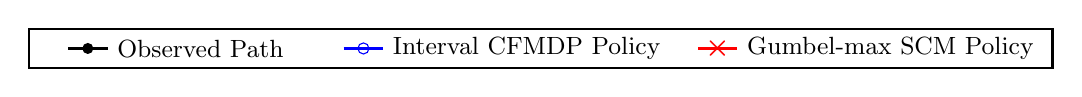
\begin{tikzpicture}[scale=1.0, every node/.style={scale=1.0}]
            \draw[thick, black] (-3, -0.25) rectangle (10, 0.25);
            %
            \draw[black, line width=1pt] (-2.5, 0.0) -- (-2,0.0);
            \fill[black] (-2.25,0.0) circle (2pt); %
            \node[right] at (-2,0.0) {\small Observed Path};
            
            %
            \draw[blue, line width=1pt] (1.0,0.0) -- (1.5,0.0);
            \node[draw=blue, circle, minimum size=4pt, inner sep=0pt] at (1.25,0.0) {}; %
            \node[right] at (1.5,0.0) {\small Interval CFMDP Policy};
            
            %
            \draw[red, line width=1pt] (5.5,0) -- (6,0);
            \node[red] at (5.75,0) {$\boldsymbol{\times}$}; %
            \node[right] at (6,0) {\small Gumbel-max SCM Policy};
        \end{tikzpicture}
    }\\
    %
    \subfigure[\footnotesize Lowest cumulative reward: Interval CFMDP ($312$), Gumbel-max SCM ($312$)]{%
        \resizebox{0.76\columnwidth}{!}{
             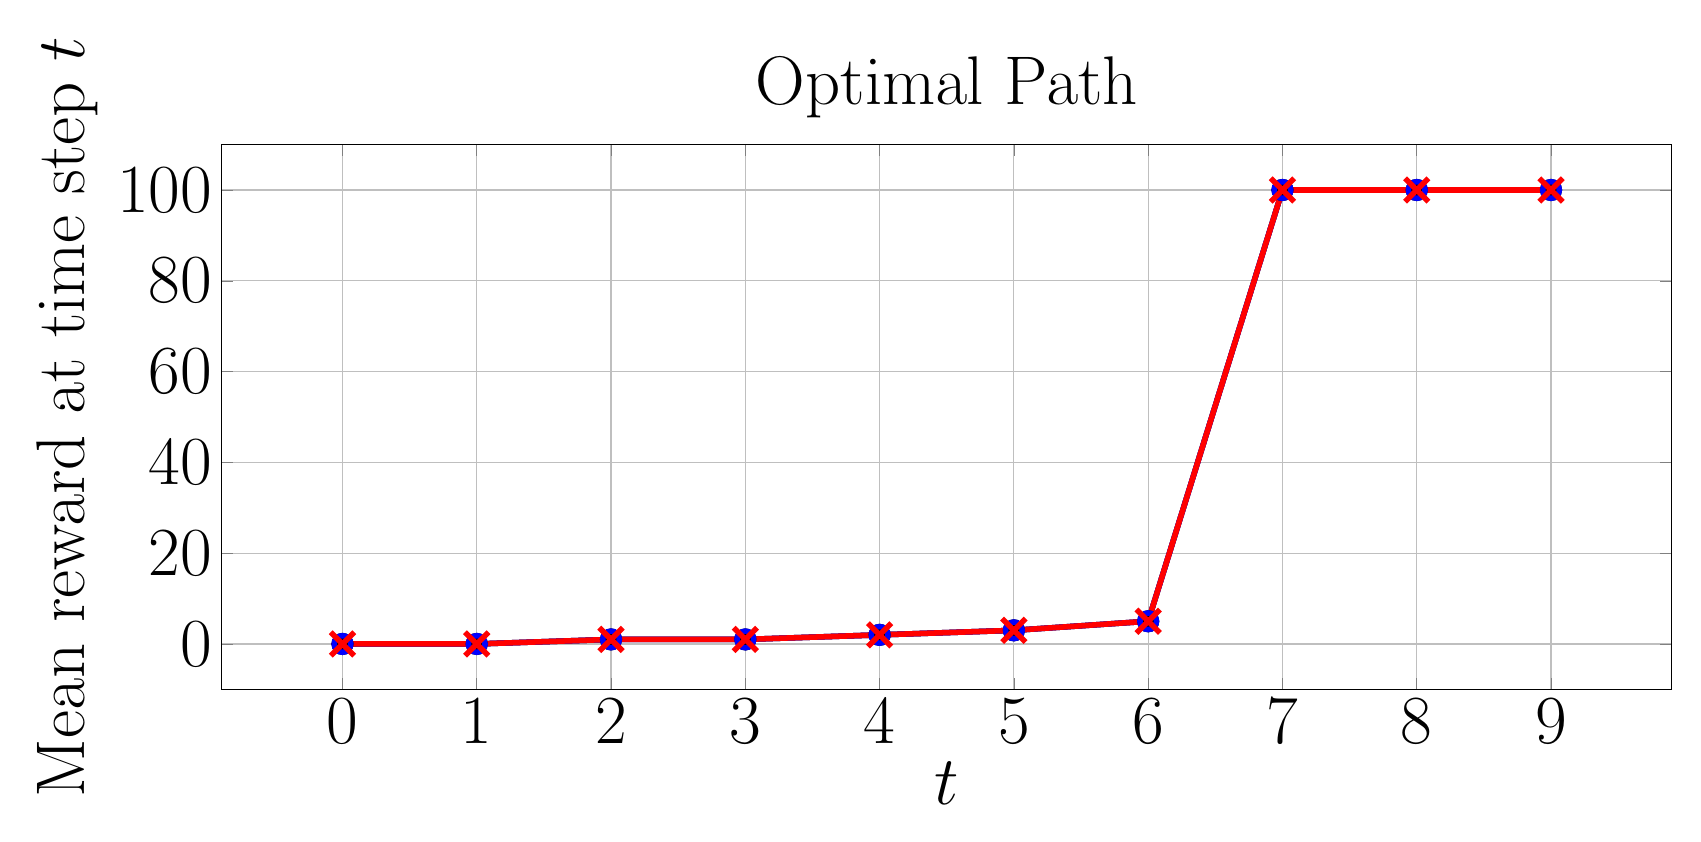
\begin{tikzpicture}
                \begin{axis}[
                    xlabel={$t$},
                    ylabel={Mean reward at time step $t$},
                    title={Optimal Path},
                    grid=both,
                    width=20cm, height=8.5cm,
                    every axis/.style={font=\Huge},
                    %
                ]
                \addplot[
                    color=black, %
                    mark=*, %
                    line width=2pt,
                    mark size=3pt,
                    error bars/.cd,
                    y dir=both, %
                    y explicit, %
                    error bar style={line width=1pt,solid},
                    error mark options={line width=1pt,mark size=4pt,rotate=90}
                ]
                coordinates {
                    (0, 0.0)  +- (0, 0.0)
                    (1, 0.0)  +- (0, 0.0) 
                    (2, 1.0)  +- (0, 0.0) 
                    (3, 1.0)  +- (0, 0.0)
                    (4, 2.0)  +- (0, 0.0)
                    (5, 3.0) +- (0, 0.0)
                    (6, 5.0) +- (0, 0.0)
                    (7, 100.0) +- (0, 0.0)
                    (8, 100.0) +- (0, 0.0)
                    (9, 100.0) +- (0, 0.0)
                };
                %
                \addplot[
                    color=blue, %
                    mark=o, %
                    line width=2pt,
                    mark size=3pt,
                    error bars/.cd,
                    y dir=both, %
                    y explicit, %
                    error bar style={line width=1pt,solid},
                    error mark options={line width=1pt,mark size=4pt,rotate=90}
                ]
                 coordinates {
                    (0, 0.0)  +- (0, 0.0)
                    (1, 0.0)  +- (0, 0.0) 
                    (2, 1.0)  +- (0, 0.0) 
                    (3, 1.0)  +- (0, 0.0)
                    (4, 2.0)  +- (0, 0.0)
                    (5, 3.0) +- (0, 0.0)
                    (6, 5.0) +- (0, 0.0)
                    (7, 100.0) +- (0, 0.0)
                    (8, 100.0) +- (0, 0.0)
                    (9, 100.0) +- (0, 0.0)
                };
                %
                \addplot[
                    color=red, %
                    mark=x, %
                    line width=2pt,
                    mark size=6pt,
                    error bars/.cd,
                    y dir=both, %
                    y explicit, %
                    error bar style={line width=1pt,solid},
                    error mark options={line width=1pt,mark size=4pt,rotate=90}
                ]
                coordinates {
                    (0, 0.0)  +- (0, 0.0)
                    (1, 0.0)  +- (0, 0.0) 
                    (2, 1.0)  +- (0, 0.0) 
                    (3, 1.0)  +- (0, 0.0)
                    (4, 2.0)  +- (0, 0.0)
                    (5, 3.0) +- (0, 0.0)
                    (6, 5.0) +- (0, 0.0)
                    (7, 100.0) +- (0, 0.0)
                    (8, 100.0) +- (0, 0.0)
                    (9, 100.0) +- (0, 0.0)
                };
                \end{axis}
            \end{tikzpicture}
         }
    }
    \hspace{1cm}
    \subfigure[\footnotesize Lowest cumulative reward: Interval CFMDP ($19$), Gumbel-max SCM ($-88$)]{%
         \resizebox{0.76\columnwidth}{!}{
            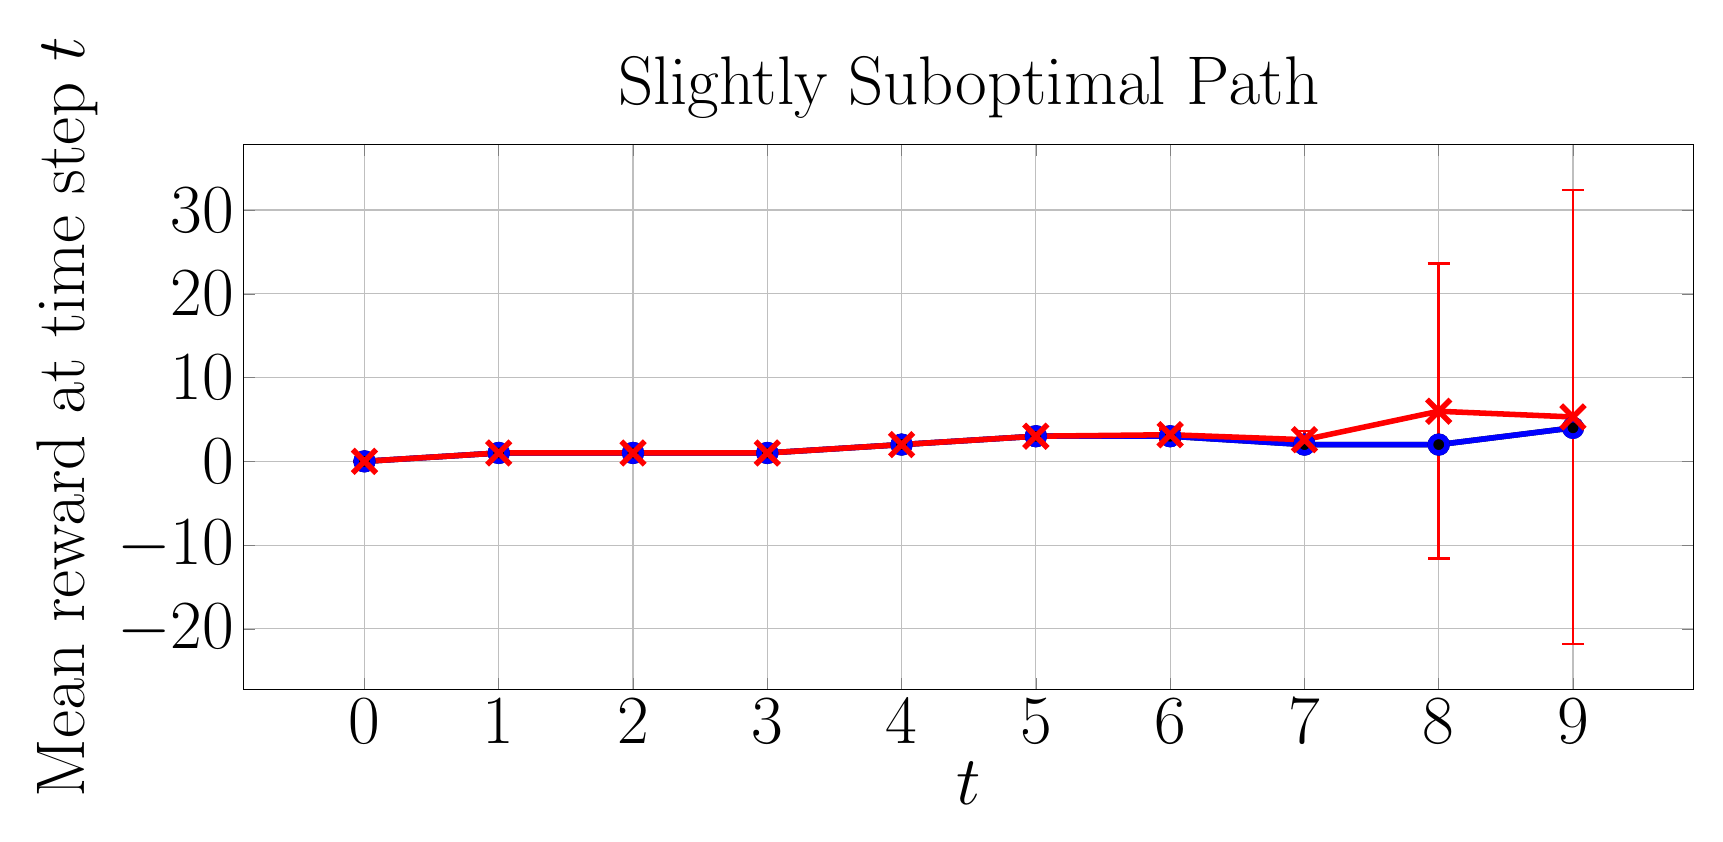
\begin{tikzpicture}
                \begin{axis}[
                    xlabel={$t$},
                    ylabel={Mean reward at time step $t$},
                    title={Slightly Suboptimal Path},
                    grid=both,
                    width=20cm, height=8.5cm,
                    every axis/.style={font=\Huge},
                    %
                ]
                \addplot[
                    color=black, %
                    mark=*, %
                    line width=2pt,
                    mark size=3pt,
                    error bars/.cd,
                    y dir=both, %
                    y explicit, %
                    error bar style={line width=1pt,solid},
                    error mark options={line width=1pt,mark size=4pt,rotate=90}
                ]
              coordinates {
                    (0, 0.0)  +- (0, 0.0)
                    (1, 1.0)  +- (0, 0.0) 
                    (2, 1.0)  +- (0, 0.0) 
                    (3, 1.0)  +- (0, 0.0)
                    (4, 2.0)  +- (0, 0.0)
                    (5, 3.0) +- (0, 0.0)
                    (6, 3.0) +- (0, 0.0)
                    (7, 2.0) +- (0, 0.0)
                    (8, 2.0) +- (0, 0.0)
                    (9, 4.0) +- (0, 0.0)
                };
                %
                \addplot[
                    color=blue, %
                    mark=o, %
                    line width=2pt,
                    mark size=3pt,
                    error bars/.cd,
                    y dir=both, %
                    y explicit, %
                    error bar style={line width=1pt,solid},
                    error mark options={line width=1pt,mark size=4pt,rotate=90}
                ]
              coordinates {
                    (0, 0.0)  +- (0, 0.0)
                    (1, 1.0)  +- (0, 0.0) 
                    (2, 1.0)  +- (0, 0.0) 
                    (3, 1.0)  +- (0, 0.0)
                    (4, 2.0)  +- (0, 0.0)
                    (5, 3.0) +- (0, 0.0)
                    (6, 3.0) +- (0, 0.0)
                    (7, 2.0) +- (0, 0.0)
                    (8, 2.0) +- (0, 0.0)
                    (9, 4.0) +- (0, 0.0)
                };
                %
                \addplot[
                    color=red, %
                    mark=x, %
                    line width=2pt,
                    mark size=6pt,
                    error bars/.cd,
                    y dir=both, %
                    y explicit, %
                    error bar style={line width=1pt,solid},
                    error mark options={line width=1pt,mark size=4pt,rotate=90}
                ]
                coordinates {
                    (0, 0.0)  +- (0, 0.0)
                    (1, 1.0)  +- (0, 0.0) 
                    (2, 1.0)  +- (0, 0.0) 
                    (3, 1.0)  +- (0, 0.0)
                    (4, 2.0)  += (0, 0.0)
                    (5, 3.0)  += (0, 0.0)
                    (6, 3.17847) += (0, 0.62606746) -= (0, 0.62606746)
                    (7, 2.5832885) += (0, 1.04598233) -= (0, 1.04598233)
                    (8, 5.978909) += (0, 17.60137623) -= (0, 17.60137623)
                    (9, 5.297059) += (0, 27.09227512) -= (0, 27.09227512)
                };
                \end{axis}
            \end{tikzpicture}
         }
    }\\[-1.5pt]
    \subfigure[\footnotesize Lowest cumulative reward: Interval CFMDP ($14$), Gumbel-max SCM ($-598$)]{%
         \resizebox{0.76\columnwidth}{!}{
             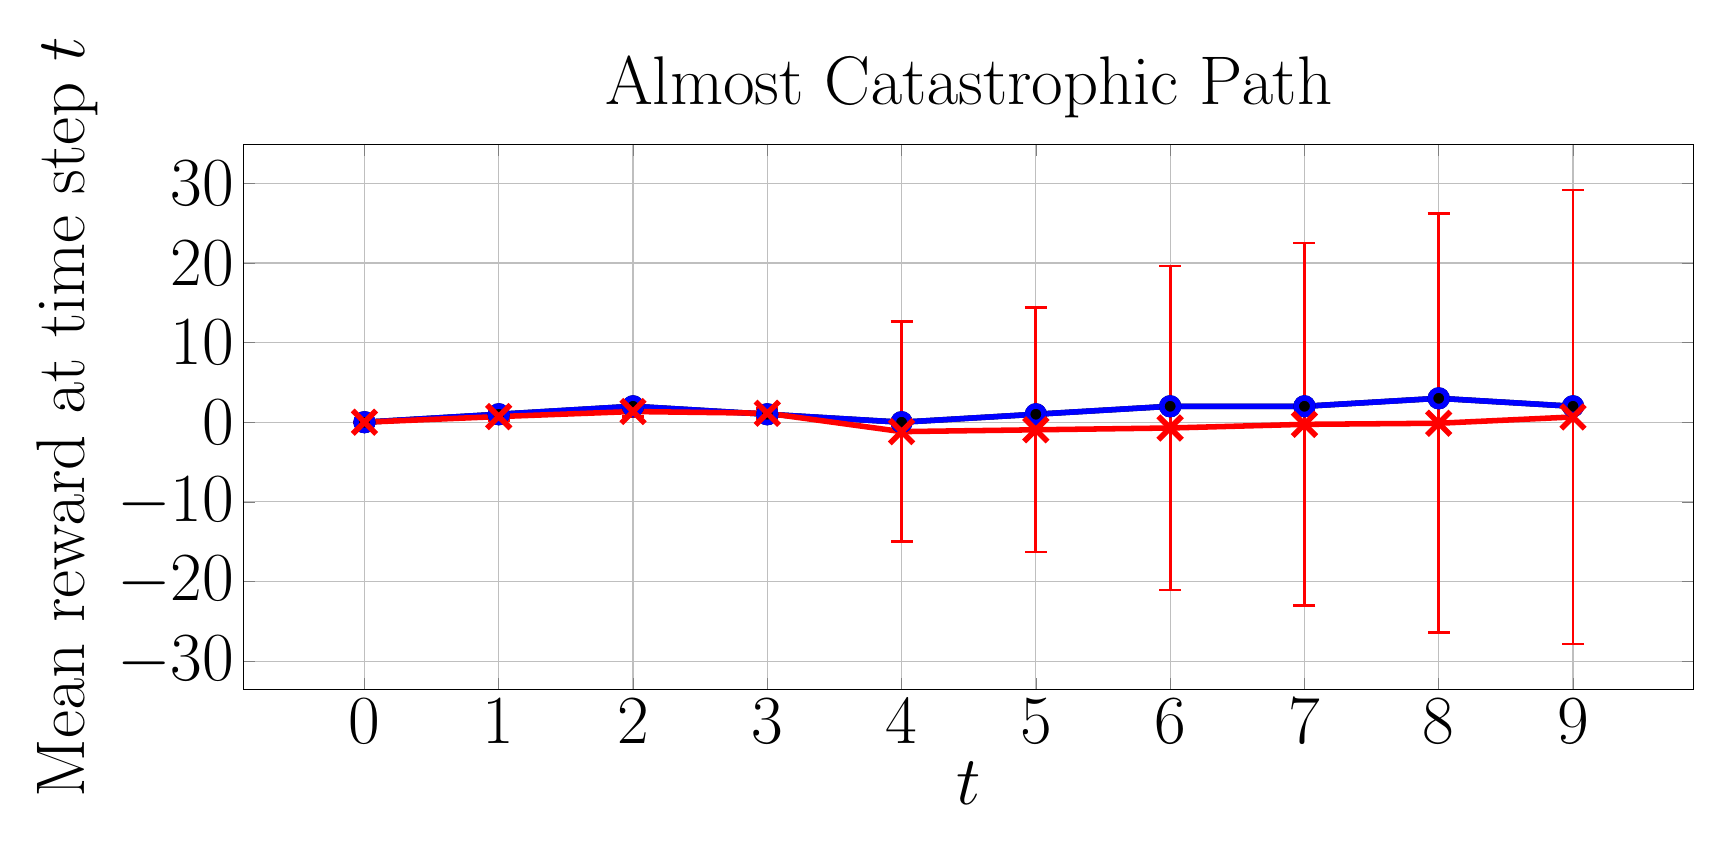
\begin{tikzpicture}
                \begin{axis}[
                    xlabel={$t$},
                    ylabel={Mean reward at time step $t$},
                    title={Almost Catastrophic Path},
                    grid=both,
                    width=20cm, height=8.5cm,
                    every axis/.style={font=\Huge},
                    %
                ]
                \addplot[
                    color=black, %
                    mark=*, %
                    line width=2pt,
                    mark size=3pt,
                    error bars/.cd,
                    y dir=both, %
                    y explicit, %
                    error bar style={line width=1pt,solid},
                    error mark options={line width=1pt,mark size=4pt,rotate=90}
                ]
                coordinates {
                    (0, 0.0)  +- (0, 0.0)
                    (1, 1.0)  +- (0, 0.0) 
                    (2, 2.0)  +- (0, 0.0) 
                    (3, 1.0)  +- (0, 0.0)
                    (4, 0.0)  +- (0, 0.0)
                    (5, 1.0) +- (0, 0.0)
                    (6, 2.0) +- (0, 0.0)
                    (7, 2.0) +- (0, 0.0)
                    (8, 3.0) +- (0, 0.0)
                    (9, 2.0) +- (0, 0.0)
                };
                %
                \addplot[
                    color=blue, %
                    mark=o, %
                    line width=2pt,
                    mark size=3pt,
                    error bars/.cd,
                    y dir=both, %
                    y explicit, %
                    error bar style={line width=1pt,solid},
                    error mark options={line width=1pt,mark size=4pt,rotate=90}
                ]
                coordinates {
                    (0, 0.0)  +- (0, 0.0)
                    (1, 1.0)  +- (0, 0.0) 
                    (2, 2.0)  +- (0, 0.0) 
                    (3, 1.0)  +- (0, 0.0)
                    (4, 0.0)  +- (0, 0.0)
                    (5, 1.0) +- (0, 0.0)
                    (6, 2.0) +- (0, 0.0)
                    (7, 2.0) +- (0, 0.0)
                    (8, 3.0) +- (0, 0.0)
                    (9, 2.0) +- (0, 0.0)
                };
                %
                \addplot[
                    color=red, %
                    mark=x, %
                    line width=2pt,
                    mark size=6pt,
                    error bars/.cd,
                    y dir=both, %
                    y explicit, %
                    error bar style={line width=1pt,solid},
                    error mark options={line width=1pt,mark size=4pt,rotate=90}
                ]
                coordinates {
                    (0, 0.0)  +- (0, 0.0)
                    (1, 0.7065655)  +- (0, 0.4553358) 
                    (2, 1.341673)  +- (0, 0.67091621) 
                    (3, 1.122926)  +- (0, 0.61281824)
                    (4, -1.1821935)  +- (0, 13.82444042)
                    (5, -0.952399)  +- (0, 15.35195457)
                    (6, -0.72672) +- (0, 20.33508414)
                    (7, -0.268983) +- (0, 22.77861454)
                    (8, -0.1310835) +- (0, 26.31013314)
                    (9, 0.65806) +- (0, 28.50670214)
                };
                %
            %
            %
            %
            %
            %
            %
            %
            %
            %
            %
            %
            %
            %
            %
            %
            %
            %
            %
                \end{axis}
            \end{tikzpicture}
         }
    }
    \hspace{1cm}
    \subfigure[\footnotesize Lowest cumulative reward: Interval CFMDP ($-698$), Gumbel-max SCM ($-698$)]{%
         \resizebox{0.76\columnwidth}{!}{
            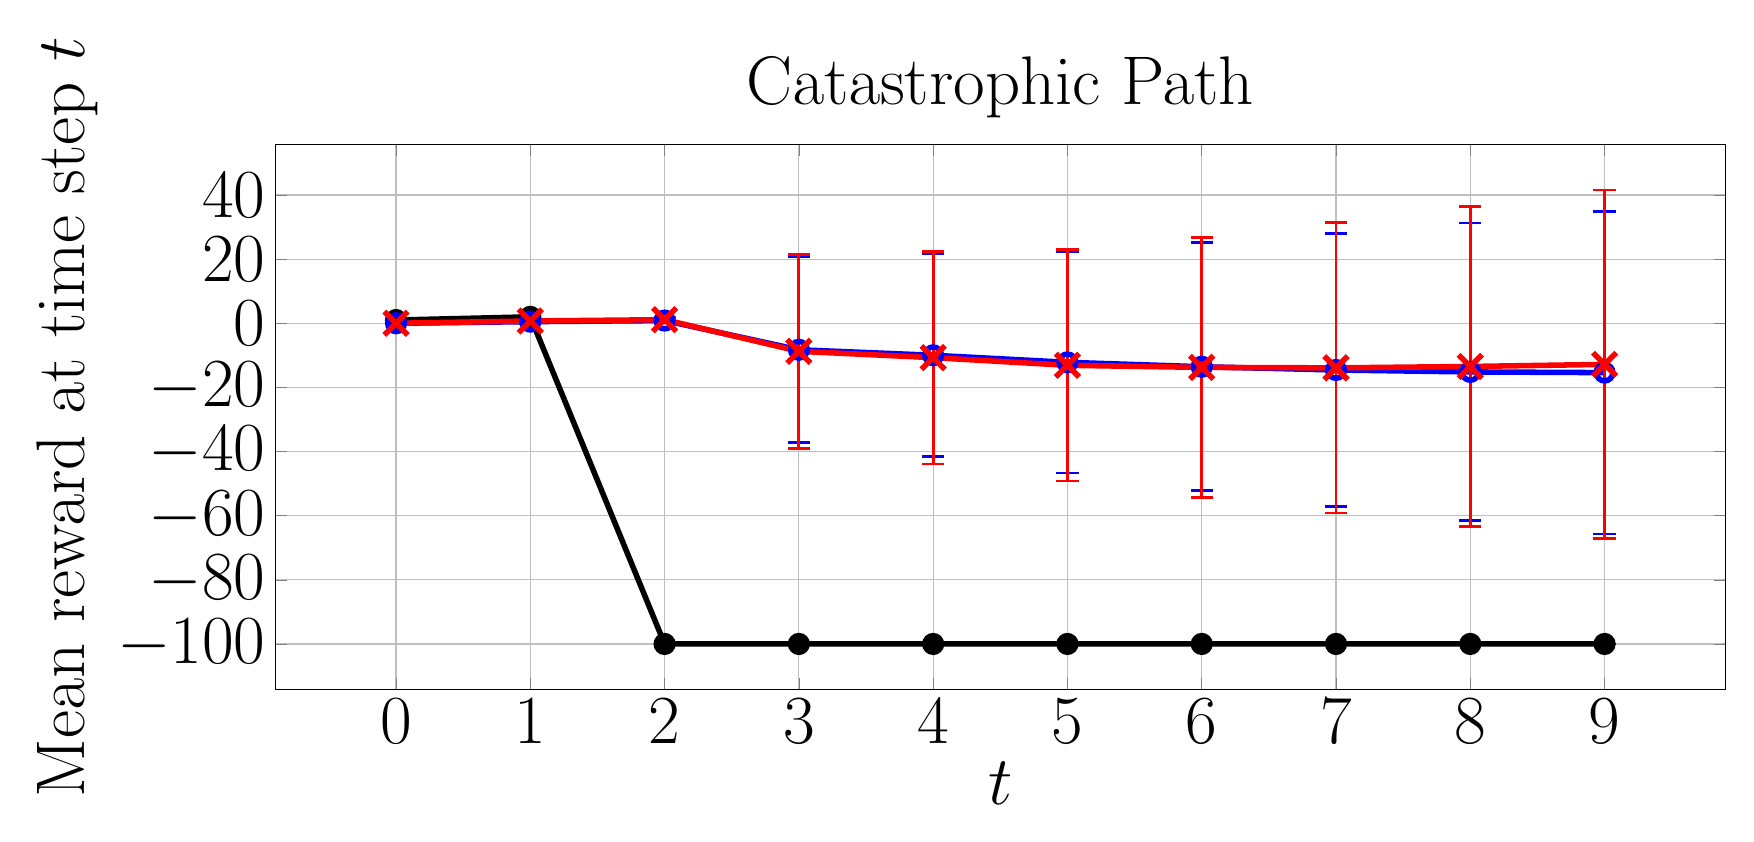
\begin{tikzpicture}
                \begin{axis}[
                    xlabel={$t$},
                    ylabel={Mean reward at time step $t$},
                    title={Catastrophic Path},
                    grid=both,
                    width=20cm, height=8.5cm,
                    every axis/.style={font=\Huge},
                    %
                ]
                \addplot[
                    color=black, %
                    mark=*, %
                    line width=2pt,
                    mark size=3pt,
                    error bars/.cd,
                    y dir=both, %
                    y explicit, %
                    error bar style={line width=1pt,solid},
                    error mark options={line width=1pt,mark size=4pt,rotate=90}
                ]
                coordinates {
                    (0, 1.0)  +- (0, 0.0)
                    (1, 2.0)  +- (0, 0.0) 
                    (2, -100.0)  +- (0, 0.0) 
                    (3, -100.0)  +- (0, 0.0)
                    (4, -100.0)  +- (0, 0.0)
                    (5, -100.0) +- (0, 0.0)
                    (6, -100.0) +- (0, 0.0)
                    (7, -100.0) +- (0, 0.0)
                    (8, -100.0) +- (0, 0.0)
                    (9, -100.0) +- (0, 0.0)
                };
                %
                \addplot[
                    color=blue, %
                    mark=o, %
                    line width=2pt,
                    mark size=3pt,
                    error bars/.cd,
                    y dir=both, %
                    y explicit, %
                    error bar style={line width=1pt,solid},
                    error mark options={line width=1pt,mark size=4pt,rotate=90}
                ]
                coordinates {
                    (0, 0.0)  +- (0, 0.0)
                    (1, 0.504814)  +- (0, 0.49997682) 
                    (2, 0.8439835)  +- (0, 0.76831917) 
                    (3, -8.2709165)  +- (0, 28.93656754)
                    (4, -9.981082)  +- (0, 31.66825363)
                    (5, -12.1776325) +- (0, 34.53463233)
                    (6, -13.556076) +- (0, 38.62845372)
                    (7, -14.574418) +- (0, 42.49603359)
                    (8, -15.1757075) +- (0, 46.41913968)
                    (9, -15.3900395) +- (0, 50.33563368)
                };
                %
                \addplot[
                    color=red, %
                    mark=x, %
                    line width=2pt,
                    mark size=6pt,
                    error bars/.cd,
                    y dir=both, %
                    y explicit, %
                    error bar style={line width=1pt,solid},
                    error mark options={line width=1pt,mark size=4pt,rotate=90}
                ]
                coordinates {
                    (0, 0.0)  +- (0, 0.0)
                    (1, 0.701873)  +- (0, 0.45743556) 
                    (2, 1.1227805)  +- (0, 0.73433129) 
                    (3, -8.7503255)  +- (0, 30.30257976)
                    (4, -10.722092)  +- (0, 33.17618589)
                    (5, -13.10721)  +- (0, 36.0648089)
                    (6, -13.7631645) +- (0, 40.56553451)
                    (7, -13.909043) +- (0, 45.23829402)
                    (8, -13.472517) +- (0, 49.96270296)
                    (9, -12.8278835) +- (0, 54.38618735)
                };
                %
            %
            %
            %
            %
            %
            %
            %
            %
            %
            %
            %
            %
            %
            %
            %
            %
            %
            %
                \end{axis}
            \end{tikzpicture}
         }
    }
    \caption{Average instant reward of CF paths induced by policies on GridWorld $p=0.4$.}
    \label{fig: reward p=0.4}
\end{figure*}

\subsection{Experimental Setup}
To compare policy performance, we measure the average rewards of counterfactual paths induced by our policy and the Gumbel-max policy by uniformly sampling $200$ counterfactual MDPs from the ICFMDP and generating $10,000$ counterfactual paths over each sampled CFMDP. \jl{Since the interval CFMDP depends on the observed path, we select $4$  paths of varying optimality to evaluate how the observed path impacts the performance of both policies: an optimal path, a slightly suboptimal path that could reach the optimal reward with a few changes, a catastrophic path that enters a catastrophic, terminal state with low reward, and an almost catastrophic path that was close to entering a catastrophic state.} When measuring the average probability bound widths and execution time needed to generate the ICFMDPs, we averaged over $20$ randomly generated observed paths
\footnote{Further training details are provided in Appendix \ref{app: training details}, and the code is provided at \href{https://github.com/ddv-lab/robust-cf-inference-in-MDPs}{https://github.com/ddv-lab/robust-cf-inference-in-MDPs}
%
%
.}.

\subsection{GridWorld}
\jl{The GridWorld MDP is a $4 \times 4$ grid where an agent must navigate from the top-left corner to the goal state in the bottom-right corner, avoiding a dangerous terminal state in the centre. At each time step, the agent can move up, down, left, or right, but there is a small probability (controlled by hyper-parameter $p$) of moving in an unintended direction. As the agent nears the goal, the reward for each state increases, culminating in a reward of $+100$ for reaching the goal. Entering the dangerous state results in a penalty of $-100$. We use two versions of GridWorld: a less stochastic version with $p=0.9$ (i.e., $90$\% chance of moving in the chosen direction) and a more stochastic version with $p=0.4$.}

\paragraph{GridWorld ($p=0.9$)}
When $p=0.9$, the counterfactual probability bounds are typically narrow (see Table \ref{tab:nonzero_probs} for average measurements). Consequently, as shown in Figure \ref{fig: reward p=0.9}, both policies are nearly identical and perform similarly well across the optimal, slightly suboptimal, and catastrophic paths.
%
However, for the almost catastrophic path, the interval CFMDP path is more conservative and follows the observed path more closely (as this is where the probability bounds are narrowest), which typically requires one additional step to reach the goal state than the Gumbel-max SCM policy.
%

\paragraph{GridWorld ($p=0.4$)}
\jl{When $p=0.4$, the GridWorld environment becomes more uncertain, increasing the risk of entering the dangerous state even if correct actions are chosen. Thus, as shown in Figure \ref{fig: reward p=0.4}, the interval CFMDP policy adopts a more conservative approach, avoiding deviation from the observed policy if it cannot guarantee higher counterfactual rewards (see the slightly suboptimal and almost catastrophic paths), whereas the Gumbel-max SCM is inconsistent: it can yield higher rewards, but also much lower rewards, reflected in the wide error bars.} For the catastrophic path, both policies must deviate from the observed path to achieve a higher reward and, in this case, perform similarly.
%
%
%
%
\subsection{Sepsis}
The Sepsis MDP \citep{oberst2019counterfactual} simulates trajectories of Sepsis patients. Each state consists of four vital signs (heart rate, blood pressure, oxygen concentration, and glucose levels), categorised as low, normal, or high.
and three treatments that can be toggled on/off at each time step (8 actions in total). Unlike \citet{oberst2019counterfactual}, we scale rewards based on the number of out-of-range vital signs, between $-1000$ (patient dies) and $1000$ (patient discharged). \jl{Like the GridWorld $p=0.4$ experiment, the Sepsis MDP is highly uncertain, as many states are equally likely to lead to optimal and poor outcomes. Thus, as shown in Figure \ref{fig: reward sepsis}, both policies follow the observed optimal and almost catastrophic paths to guarantee rewards are no worse than the observation.} However, improving the catastrophic path requires deviating from the observation. Here, the Gumbel-max SCM policy, on average, performs better than the interval CFMDP policy. But, since both policies have lower bounds clipped at $-1000$, neither policy reliably improves over the observation. In contrast, for the slightly suboptimal path, the interval CFMDP policy performs significantly better, shown by its higher lower bounds. 
Moreover, in these two cases, the worst-case counterfactual path generated by the interval CFMDP policy is better than that of the Gumbel-max SCM policy,
indicating its greater robustness.
%
\begin{figure*}
    \centering
     \resizebox{0.6\textwidth}{!}{
        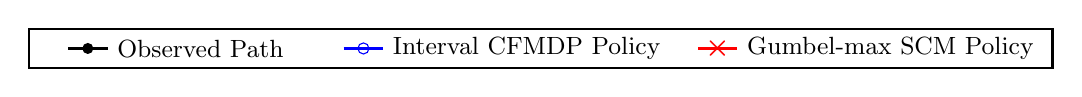
\begin{tikzpicture}[scale=1.0, every node/.style={scale=1.0}]
            \draw[thick, black] (-3, -0.25) rectangle (10, 0.25);
            %
            \draw[black, line width=1pt] (-2.5, 0.0) -- (-2,0.0);
            \fill[black] (-2.25,0.0) circle (2pt); %
            \node[right] at (-2,0.0) {\small Observed Path};
            
            %
            \draw[blue, line width=1pt] (1.0,0.0) -- (1.5,0.0);
            \node[draw=blue, circle, minimum size=4pt, inner sep=0pt] at (1.25,0.0) {}; %
            \node[right] at (1.5,0.0) {\small Interval CFMDP Policy};
            
            %
            \draw[red, line width=1pt] (5.5,0) -- (6,0);
            \node[red] at (5.75,0) {$\boldsymbol{\times}$}; %
            \node[right] at (6,0) {\small Gumbel-max SCM Policy};
        \end{tikzpicture}
    }\\
    \subfigure[\footnotesize Lowest cumulative reward: Interval CFMDP ($8000$), Gumbel-max SCM ($8000$)]{%
         \resizebox{0.76\columnwidth}{!}{
             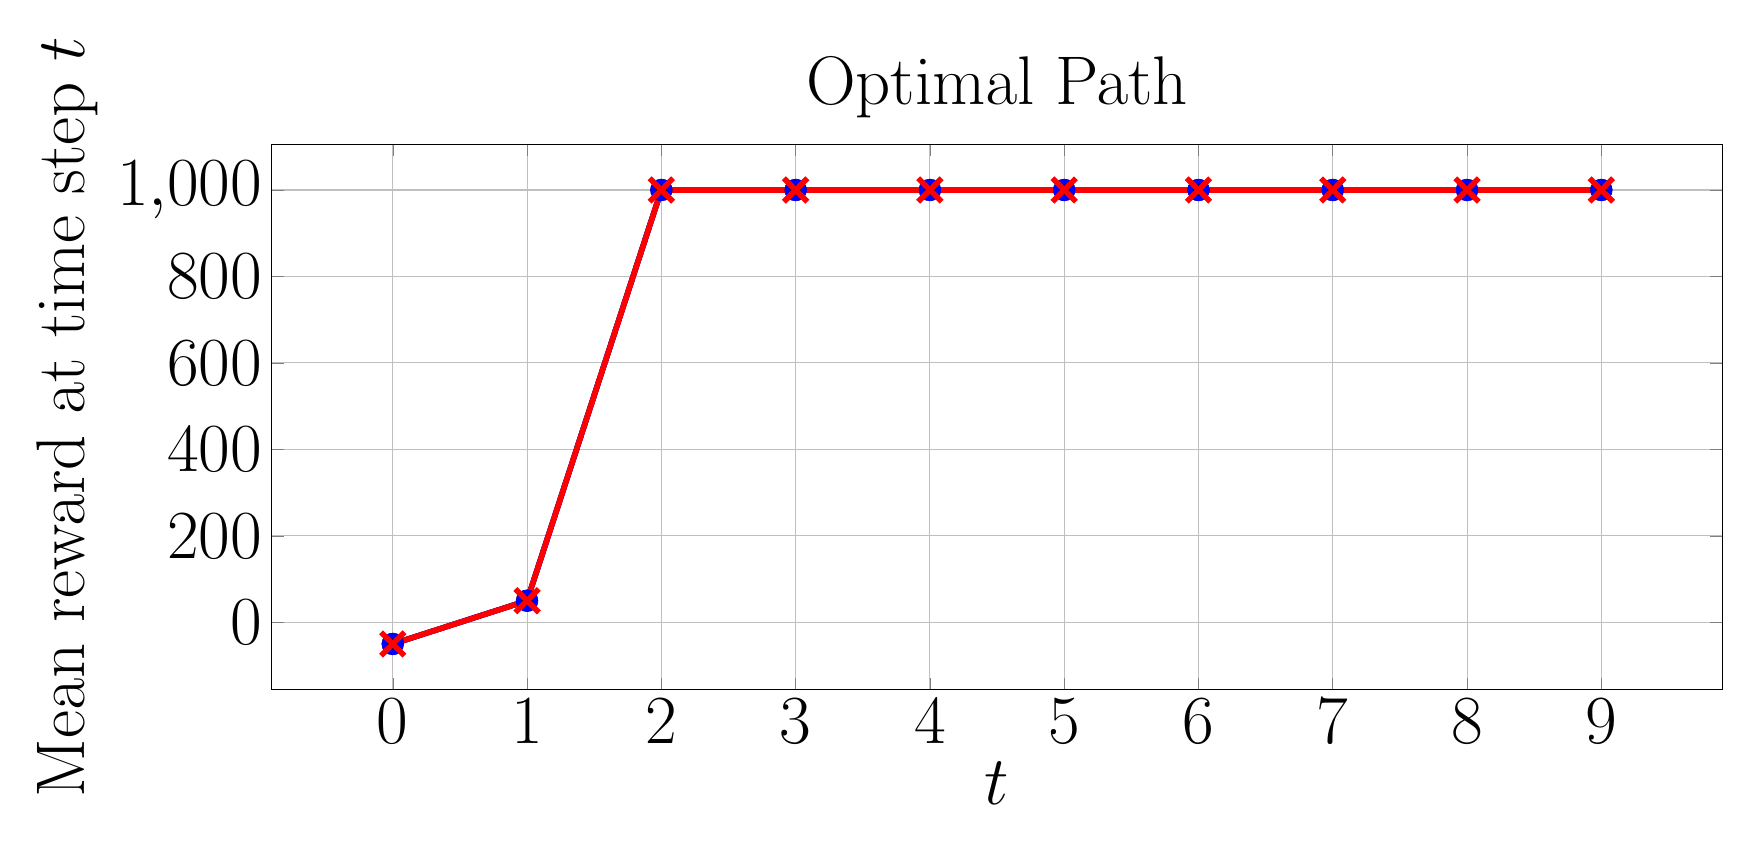
\begin{tikzpicture}
                \begin{axis}[
                    xlabel={$t$},
                    ylabel={Mean reward at time step $t$},
                    title={Optimal Path},
                    grid=both,
                    width=20cm, height=8.5cm,
                    every axis/.style={font=\Huge},
                    %
                ]
                \addplot[
                    color=black, %
                    mark=*, %
                    line width=2pt,
                    mark size=3pt,
                ]
                coordinates {
                    (0, -50.0)
                    (1, 50.0)
                    (2, 1000.0)
                    (3, 1000.0)
                    (4, 1000.0)
                    (5, 1000.0)
                    (6, 1000.0)
                    (7, 1000.0)
                    (8, 1000.0)
                    (9, 1000.0)
                };
                %
                \addplot[
                    color=blue, %
                    mark=o, %
                    line width=2pt,
                    mark size=3pt,
                    error bars/.cd,
                    y dir=both, %
                    y explicit, %
                    error bar style={line width=1pt,solid},
                    error mark options={line width=1pt,mark size=4pt,rotate=90}
                ]
                coordinates {
                    (0, -50.0)  +- (0, 0.0)
                    (1, 50.0)  +- (0, 0.0) 
                    (2, 1000.0)  +- (0, 0.0) 
                    (3, 1000.0)  +- (0, 0.0)
                    (4, 1000.0)  +- (0, 0.0)
                    (5, 1000.0) +- (0, 0.0)
                    (6, 1000.0) +- (0, 0.0)
                    (7, 1000.0) +- (0, 0.0)
                    (8, 1000.0) +- (0, 0.0)
                    (9, 1000.0) +- (0, 0.0)
                };
                %
                \addplot[
                    color=red, %
                    mark=x, %
                    line width=2pt,
                    mark size=6pt,
                    error bars/.cd,
                    y dir=both, %
                    y explicit, %
                    error bar style={line width=1pt,solid},
                    error mark options={line width=1pt,mark size=4pt,rotate=90}
                ]
                coordinates {
                    (0, -50.0)  +- (0, 0.0)
                    (1, 50.0)  +- (0, 0.0) 
                    (2, 1000.0)  +- (0, 0.0) 
                    (3, 1000.0)  +- (0, 0.0)
                    (4, 1000.0)  +- (0, 0.0)
                    (5, 1000.0) +- (0, 0.0)
                    (6, 1000.0) +- (0, 0.0)
                    (7, 1000.0) +- (0, 0.0)
                    (8, 1000.0) +- (0, 0.0)
                    (9, 1000.0) +- (0, 0.0)
                };
                %
                \end{axis}
            \end{tikzpicture}
         }
    }
    \hspace{1cm}
    \subfigure[\footnotesize Lowest cumulative reward: Interval CFMDP ($-5980$), Gumbel-max SCM ($-8000$)]{%
         \resizebox{0.76\columnwidth}{!}{
            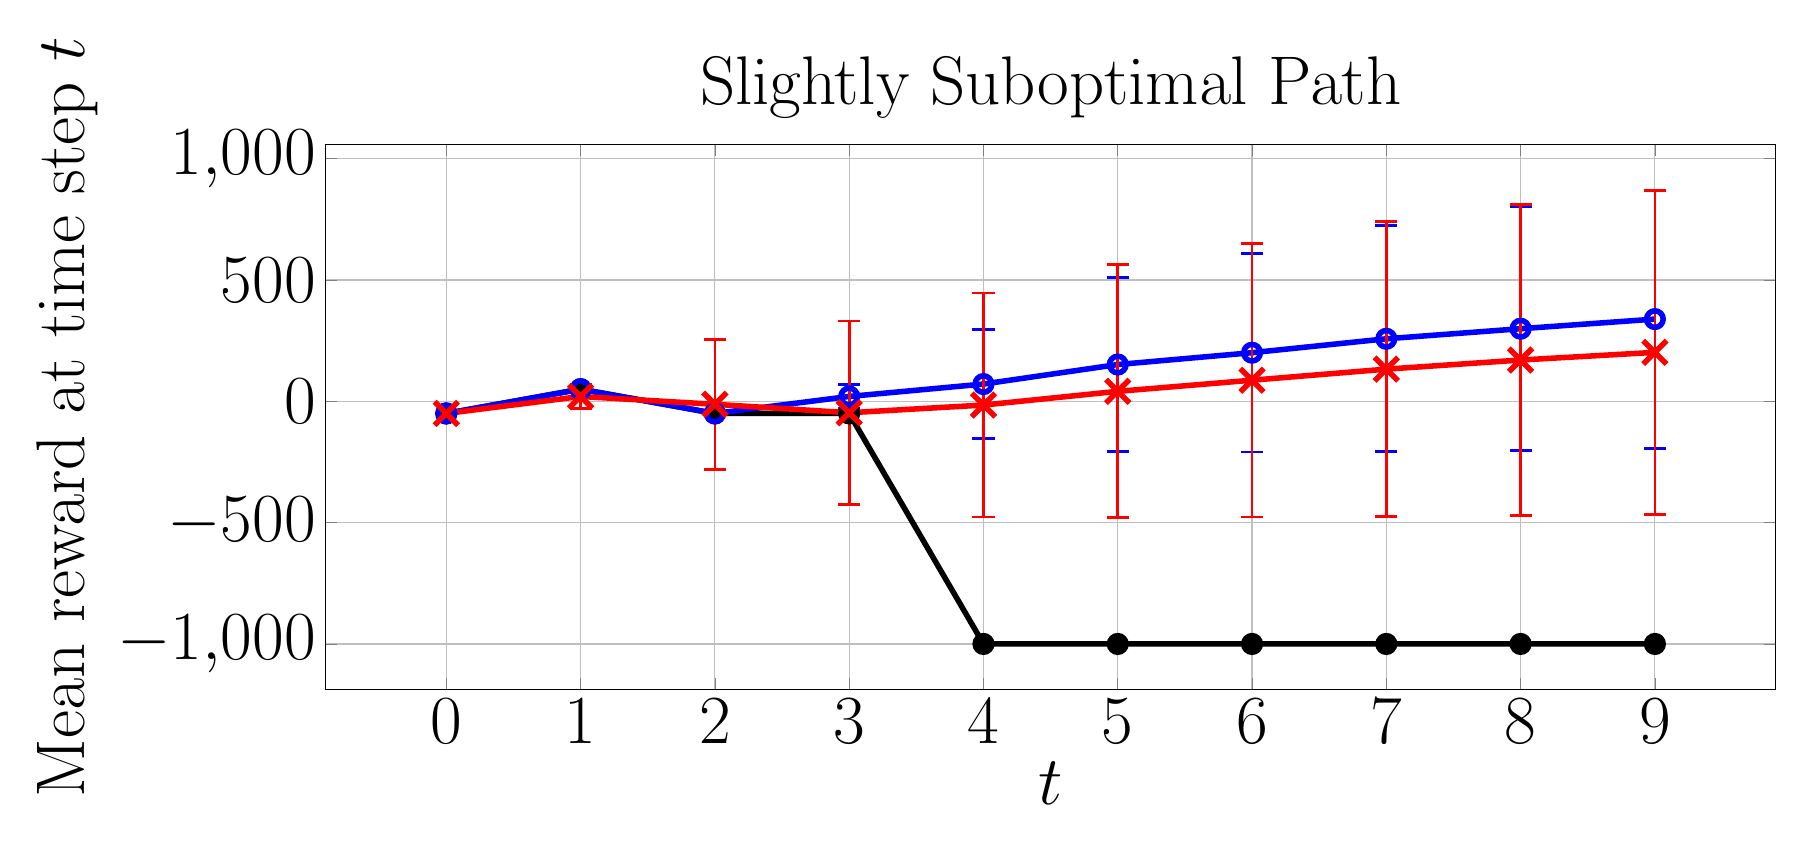
\begin{tikzpicture}
                \begin{axis}[
                    xlabel={$t$},
                    ylabel={Mean reward at time step $t$},
                    title={Slightly Suboptimal Path},
                    grid=both,
                    width=20cm, height=8.5cm,
                    every axis/.style={font=\Huge},
                    %
                ]
               \addplot[
                    color=black, %
                    mark=*, %
                    line width=2pt,
                    mark size=3pt,
                ]
                coordinates {
                    (0, -50.0)
                    (1, 50.0)
                    (2, -50.0)
                    (3, -50.0)
                    (4, -1000.0)
                    (5, -1000.0)
                    (6, -1000.0)
                    (7, -1000.0)
                    (8, -1000.0)
                    (9, -1000.0)
                };
                %
                \addplot[
                    color=blue, %
                    mark=o, %
                    line width=2pt,
                    mark size=3pt,
                    error bars/.cd,
                    y dir=both, %
                    y explicit, %
                    error bar style={line width=1pt,solid},
                    error mark options={line width=1pt,mark size=4pt,rotate=90}
                ]
                coordinates {
                    (0, -50.0)  +- (0, 0.0)
                    (1, 50.0)  +- (0, 0.0) 
                    (2, -50.0)  +- (0, 0.0) 
                    (3, 20.0631)  +- (0, 49.97539413)
                    (4, 71.206585)  +- (0, 226.02033693)
                    (5, 151.60797) +- (0, 359.23292559)
                    (6, 200.40593) +- (0, 408.86185176)
                    (7, 257.77948) +- (0, 466.10372804)
                    (8, 299.237465) +- (0, 501.82579506)
                    (9, 338.9129) +- (0, 532.06124996)
                };
                %
                \addplot[
                    color=red, %
                    mark=x, %
                    line width=2pt,
                    mark size=6pt,
                    error bars/.cd,
                    y dir=both, %
                    y explicit, %
                    error bar style={line width=1pt,solid},
                    error mark options={line width=1pt,mark size=4pt,rotate=90}
                ]
                coordinates {
                    (0, -50.0)  +- (0, 0.0)
                    (1, 20.00736)  +- (0, 49.99786741) 
                    (2, -12.282865)  +- (0, 267.598755) 
                    (3, -47.125995)  +- (0, 378.41755832)
                    (4, -15.381965)  +- (0, 461.77616558)
                    (5, 41.15459) +- (0, 521.53189262)
                    (6, 87.01595) +- (0, 564.22243126 )
                    (7, 132.62376) +- (0, 607.31338037)
                    (8, 170.168145) +- (0, 641.48013693)
                    (9, 201.813135) +- (0, 667.29441777)
                };
                %
                %
                %
                %
                %
                %
                %
                %
                %
                %
                %
                %
                %
                %
                %
                %
                %
                %
                %
                \end{axis}
            \end{tikzpicture}
         }
    }\\[-1.5pt]
    \subfigure[\footnotesize Lowest cumulative reward: Interval CFMDP ($100$), Gumbel-max SCM ($100$)]{%
         \resizebox{0.76\columnwidth}{!}{
             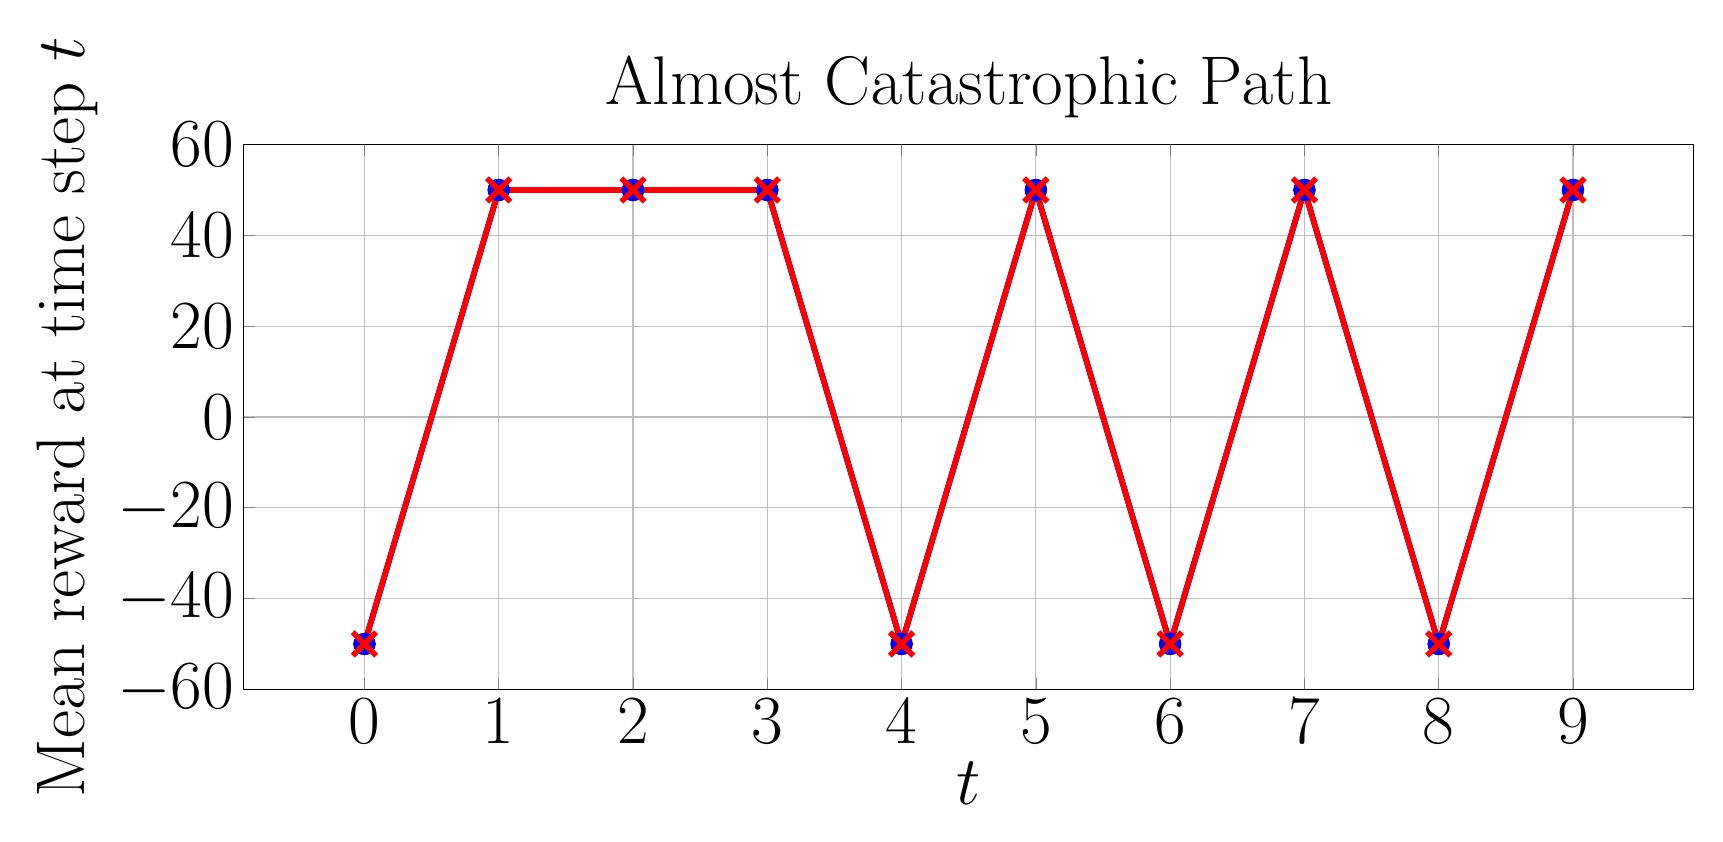
\begin{tikzpicture}
                \begin{axis}[
                    xlabel={$t$},
                    ylabel={Mean reward at time step $t$},
                    title={Almost Catastrophic Path},
                    grid=both,
                    every axis/.style={font=\Huge},
                    width=20cm, height=8.5cm,
                    %
                ]
               \addplot[
                    color=black, %
                    mark=*, %
                    line width=2pt,
                    mark size=3pt,
                ]
                coordinates {
                    (0, -50.0)
                    (1, 50.0)
                    (2, 50.0)
                    (3, 50.0)
                    (4, -50.0)
                    (5, 50.0)
                    (6, -50.0)
                    (7, 50.0)
                    (8, -50.0)
                    (9, 50.0)
                };
                %
                %
                \addplot[
                    color=blue, %
                    mark=o, %
                    line width=2pt,
                    mark size=3pt,
                    error bars/.cd,
                    y dir=both, %
                    y explicit, %
                    error bar style={line width=1pt,solid},
                    error mark options={line width=1pt,mark size=4pt,rotate=90}
                ]
                coordinates {
                    (0, -50.0)  +- (0, 0.0)
                    (1, 50.0)  +- (0, 0.0) 
                    (2, 50.0)  +- (0, 0.0) 
                    (3, 50.0)  +- (0, 0.0)
                    (4, -50.0)  +- (0, 0.0)
                    (5, 50.0) +- (0, 0.0)
                    (6, -50.0) +- (0, 0.0)
                    (7, 50.0) +- (0, 0.0)
                    (8, -50.0) +- (0, 0.0)
                    (9, 50.0) +- (0, 0.0)
                };
                %
                \addplot[
                    color=red, %
                    mark=x, %
                    line width=2pt,
                    mark size=6pt,
                    error bars/.cd,
                    y dir=both, %
                    y explicit, %
                    error bar style={line width=1pt,solid},
                    error mark options={line width=1pt,mark size=4pt,rotate=90}
                ]
                coordinates {
                    (0, -50.0)  +- (0, 0.0)
                    (1, 50.0)  +- (0, 0.0) 
                    (2, 50.0)  +- (0, 0.0) 
                    (3, 50.0)  +- (0, 0.0)
                    (4, -50.0)  +- (0, 0.0)
                    (5, 50.0) +- (0, 0.0)
                    (6, -50.0) +- (0, 0.0)
                    (7, 50.0) +- (0, 0.0)
                    (8, -50.0) +- (0, 0.0)
                    (9, 50.0) +- (0, 0.0)
                };
                %
                %
                %
                %
                %
                %
                %
                %
                %
                %
                %
                %
                %
                %
                %
                %
                %
                %
                %
                \end{axis}
            \end{tikzpicture}
         }
    }
    \hspace{1cm}
    \subfigure[\footnotesize Lowest cumulative reward: Interval CFMDP ($-7150$), Gumbel-max SCM ($-9050$)]{%
         \resizebox{0.76\columnwidth}{!}{
            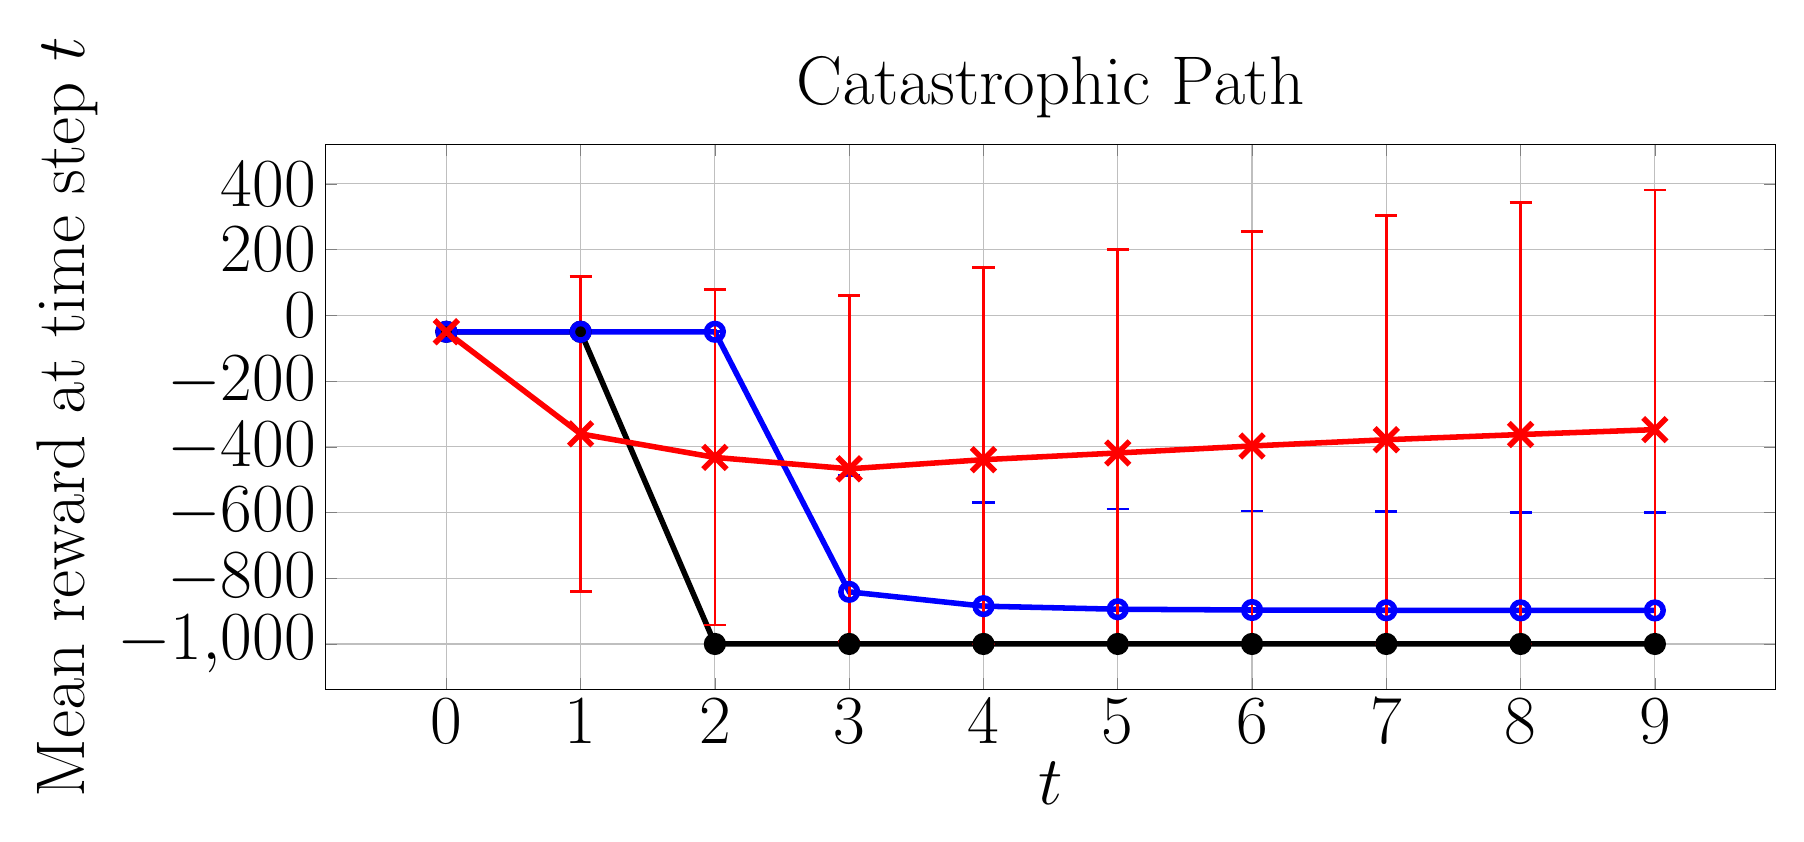
\begin{tikzpicture}
                \begin{axis}[
                    xlabel={$t$},
                    ylabel={Mean reward at time step $t$},
                    title={Catastrophic Path},
                    grid=both,
                    width=20cm, height=8.5cm,
                    every axis/.style={font=\Huge},
                    %
                ]
               \addplot[
                    color=black, %
                    mark=*, %
                    line width=2pt,
                    mark size=3pt,
                ]
                coordinates {
                    (0, -50.0)
                    (1, -50.0)
                    (2, -1000.0)
                    (3, -1000.0)
                    (4, -1000.0)
                    (5, -1000.0)
                    (6, -1000.0)
                    (7, -1000.0)
                    (8, -1000.0)
                    (9, -1000.0)
                };
                %
                %
                \addplot[
                    color=blue, %
                    mark=o, %
                    line width=2pt,
                    mark size=3pt,
                    error bars/.cd,
                    y dir=both, %
                    y explicit, %
                    error bar style={line width=1pt,solid},
                    error mark options={line width=1pt,mark size=4pt,rotate=90}
                ]
                coordinates {
                    (0, -50.0)  +- (0, 0.0)
                    (1, -50.0)  +- (0, 0.0) 
                    (2, -50.0)  +- (0, 0.0) 
                    (3, -841.440725)  += (0, 354.24605512) -= (0, 158.559275)
                    (4, -884.98225)  += (0, 315.37519669) -= (0, 115.01775)
                    (5, -894.330425) += (0, 304.88572805) -= (0, 105.669575)
                    (6, -896.696175) += (0, 301.19954514) -= (0, 103.303825)
                    (7, -897.4635) += (0, 299.61791279) -= (0, 102.5365)
                    (8, -897.77595) += (0, 298.80392585) -= (0, 102.22405)
                    (9, -897.942975) += (0, 298.32920557) -= (0, 102.057025)
                };
                %
                \addplot[
                    color=red, %
                    mark=x, %
                    line width=2pt,
                    mark size=6pt,
                    error bars/.cd,
                    y dir=both, %
                    y explicit, %
                    error bar style={line width=1pt,solid},
                    error mark options={line width=1pt,mark size=4pt,rotate=90}
                ]
            coordinates {
                    (0, -50.0)  +- (0, 0.0)
                    (1, -360.675265)  +- (0, 479.39812699) 
                    (2, -432.27629)  +- (0, 510.38620897) 
                    (3, -467.029545)  += (0, 526.36009628) -= (0, 526.36009628)
                    (4, -439.17429)  += (0, 583.96638919) -= (0, 560.82571)
                    (5, -418.82704) += (0, 618.43027478) -= (0, 581.17296)
                    (6, -397.464895) += (0, 652.67322574) -= (0, 602.535105)
                    (7, -378.49052) += (0, 682.85407033) -= (0, 621.50948)
                    (8, -362.654195) += (0, 707.01412023) -= (0, 637.345805)
                    (9, -347.737935) += (0, 729.29076479) -= (0, 652.262065)
                };
                %
                %
                %
                %
                %
                %
                %
                %
                %
                %
                %
                %
                %
                %
                %
                %
                %
                %
                %
                \end{axis}
            \end{tikzpicture}
         }
    }
    \caption{Average instant reward of CF paths induced by policies on Sepsis.}
    \label{fig: reward sepsis}
\end{figure*}

%
%
%
\subsection{Interval CFMDP Bounds}
%
%
Table \ref{tab:nonzero_probs} presents the mean counterfactual probability bound widths (excluding transitions where the upper bound is $0$) for each MDP, averaged over 20 observed paths. We compare the bounds under counterfactual stability (CS) and monotonicity (M) assumptions, CS alone, and no assumptions. This shows that the assumptions marginally reduce the bound widths, indicating the assumptions tighten the bounds without excluding too many causal models, as intended.
\renewcommand{\arraystretch}{1}

\begin{table}
\centering
\caption{Mean width of counterfactual probability bounds}
\resizebox{0.8\columnwidth}{!}{%
\begin{tabular}{|c|c|c|c|}
\hline
\multirow{2}{*}{\textbf{Environment}} & \multicolumn{3}{c|}{\textbf{Assumptions}} \\ \cline{2-4}
 & \textbf{CS + M} & \textbf{CS} & \textbf{None\tablefootnote{\jl{Equivalent to \citet{li2024probabilities}'s bounds (see Section \ref{sec: equivalence with Li}).}}} \\ \hline
\textbf{GridWorld} ($p=0.9$) & 0.0817 & 0.0977 & 0.100 \\ \hline
\textbf{GridWorld} ($p=0.4$) & 0.552  & 0.638  & 0.646 \\ \hline
\textbf{Sepsis} & 0.138 & 0.140 & 0.140 \\ \hline
\end{tabular}
}
\label{tab:nonzero_probs}
\end{table}


\subsection{Execution Times}
Table \ref{tab: times} compares the average time needed to generate the interval CFMDP vs.\ the Gumbel-max SCM CFMDP for 20 observations.
The GridWorld algorithms were run single-threaded, while the Sepsis experiments were run in parallel.
Generating the interval CFMDP is significantly faster as it uses exact analytical bounds, whereas the Gumbel-max CFMDP requires sampling from the Gumbel distribution to estimate counterfactual transition probabilities. \jl{Since constructing the counterfactual MDP models is the main bottleneck in both approaches, ours is more efficient overall and suitable for larger MDPs.}
\begin{table}
\centering
\caption{Mean execution time to generate CFMDPs}
\resizebox{0.99\columnwidth}{!}{%
\begin{tabular}{|c|c|c|}
\hline
\multirow{2}{*}{\textbf{Environment}} & \multicolumn{2}{c|}{\textbf{Mean Execution Time (s)}} \\ \cline{2-3} 
                                      & \textbf{Interval CFMDP} & \textbf{Gumbel-max CFMDP} \\ \hline
\textbf{GridWorld ($p=0.9$) }                  & 0.261                   & 56.1                      \\ \hline
\textbf{GridWorld ($p=0.4$)  }                 & 0.336                   & 54.5                      \\ \hline
\textbf{Sepsis}                                 & 688                     & 2940                      \\ \hline
\end{tabular}%
}
\label{tab: times}
\end{table}

\putsec{related}{Related Work}

\noindent \textbf{Efficient Radiance Field Rendering.}
%
The introduction of Neural Radiance Fields (NeRF)~\cite{mil:sri20} has
generated significant interest in efficient 3D scene representation and
rendering for radiance fields.
%
Over the past years, there has been a large amount of research aimed at
accelerating NeRFs through algorithmic or software
optimizations~\cite{mul:eva22,fri:yu22,che:fun23,sun:sun22}, and the
development of hardware
accelerators~\cite{lee:cho23,li:li23,son:wen23,mub:kan23,fen:liu24}.
%
The state-of-the-art method, 3D Gaussian splatting~\cite{ker:kop23}, has
further fueled interest in accelerating radiance field
rendering~\cite{rad:ste24,lee:lee24,nie:stu24,lee:rho24,ham:mel24} as it
employs rasterization primitives that can be rendered much faster than NeRFs.
%
However, previous research focused on software graphics rendering on
programmable cores or building dedicated hardware accelerators. In contrast,
\name{} investigates the potential of efficient radiance field rendering while
utilizing fixed-function units in graphics hardware.
%
To our knowledge, this is the first work that assesses the performance
implications of rendering Gaussian-based radiance fields on the hardware
graphics pipeline with software and hardware optimizations.

%%%%%%%%%%%%%%%%%%%%%%%%%%%%%%%%%%%%%%%%%%%%%%%%%%%%%%%%%%%%%%%%%%%%%%%%%%
\myparagraph{Enhancing Graphics Rendering Hardware.}
%
The performance advantage of executing graphics rendering on either
programmable shader cores or fixed-function units varies depending on the
rendering methods and hardware designs.
%
Previous studies have explored the performance implication of graphics hardware
design by developing simulation infrastructures for graphics
workloads~\cite{bar:gon06,gub:aam19,tin:sax23,arn:par13}.
%
Additionally, several studies have aimed to improve the performance of
special-purpose hardware such as ray tracing units in graphics
hardware~\cite{cho:now23,liu:cha21} and proposed hardware accelerators for
graphics applications~\cite{lu:hua17,ram:gri09}.
%
In contrast to these works, which primarily evaluate traditional graphics
workloads, our work focuses on improving the performance of volume rendering
workloads, such as Gaussian splatting, which require blending a huge number of
fragments per pixel.

%%%%%%%%%%%%%%%%%%%%%%%%%%%%%%%%%%%%%%%%%%%%%%%%%%%%%%%%%%%%%%%%%%%%%%%%%%
%
In the context of multi-sample anti-aliasing, prior work proposed reducing the
amount of redundant shading by merging fragments from adjacent triangles in a
mesh at the quad granularity~\cite{fat:bou10}.
%
While both our work and quad-fragment merging (QFM)~\cite{fat:bou10} aim to
reduce operations by merging quads, our proposed technique differs from QFM in
many aspects.
%
Our method aims to blend \emph{overlapping primitives} along the depth
direction and applies to quads from any primitive. In contrast, QFM merges quad
fragments from small (e.g., pixel-sized) triangles that \emph{share} an edge
(i.e., \emph{connected}, \emph{non-overlapping} triangles).
%
As such, QFM is not applicable to the scenes consisting of a number of
unconnected transparent triangles, such as those in 3D Gaussian splatting.
%
In addition, our method computes the \emph{exact} color for each pixel by
offloading blending operations from ROPs to shader units, whereas QFM
\emph{approximates} pixel colors by using the color from one triangle when
multiple triangles are merged into a single quad.



\section{Conclusion}
Training state-of-the-art LLMs requires a significant number of GPUs and enormous training data.
There have been several work driven by the need for cost-effective training where they explored communication and computation improvements over DP and PP methods. 
Yet, existing PP methods are limited to the sequential execution of the layers.
In this paper we introduced a novel approach to pipeline parallelism, \sys, which makes use of stage skips and swaps to increase throughput by up to \(55\%\) in heterogeneous network settings. Our partial training also produces models resistant to layer removals during inference, which makes them suitable for early exit and fault tolerant inference. Our LLaMa-500M model trained with \sys experiences a drop in perplexity of only 7\% when running half the model.

Finally, while this paper focuses on the homogeneous nodes/ heterogeneous network, in future work, we plan to extend our solution to the full heterogeneous setting where nodes can have different memory and computational capacities.

\section*{Acknowledgment}
This work has been supported by Gensyn. 




\bibliography{scheduling_paper}
\bibliographystyle{icml2025}


%%%%%%%%%%%%%%%%%%%%%%%%%%%%%%%%%%%%%%%%%%%%%%%%%%%%%%%%%%%%%%%%%%%%%%%%%%%%%%%
%%%%%%%%%%%%%%%%%%%%%%%%%%%%%%%%%%%%%%%%%%%%%%%%%%%%%%%%%%%%%%%%%%%%%%%%%%%%%%%
% APPENDIX
%%%%%%%%%%%%%%%%%%%%%%%%%%%%%%%%%%%%%%%%%%%%%%%%%%%%%%%%%%%%%%%%%%%%%%%%%%%%%%%
%%%%%%%%%%%%%%%%%%%%%%%%%%%%%%%%%%%%%%%%%%%%%%%%%%%%%%%%%%%%%%%%%%%%%%%%%%%%%%%
\newpage
\appendix
\onecolumn
\section{Model Configurations}
\label{appendix:mc}
\par We perform all our experiments with LLaMa-based \cite{llama} model architectures with the Sentence Piece Tokenizer \cite{SP}. The different models and their parameters are shown in Table \ref{table:models}. 

\begin{table}[h]
\caption{Model parameters.}
\label{table:models}
\begin{center}
\begin{tabular}[H]{p{6cm}p{1.2cm}p{1.2cm}p{1.2cm}p{1.2cm}}

  \toprule
  Model & Dim  & Heads & Layers & Context     \\ 
  
  \midrule
  LLaMa 50M & 288 & 6 & 12 & 256 \\
  LLaMa 500M & 1024 & 16 & 24 & 1024 \\
  LLaMa 1.5B~\cite{LayerSkip} & 2048  & 16 & 24 & 4096  \\
  LLaMa-2 7B~\cite{llama} & 4096  & 32 & 32 & 4096  \\
  LLaMa-3 8B~\cite{llama8b} & 4096  & 32 & 32 & 4096  \\
  
  \bottomrule
  

  

\end{tabular}
\end{center}
\end{table}


\section{Test Configurations}
\par Configurations of the throughput tests are presented in Table \ref{table:tests}. Stage sizes for the \(33\%\) case are (5,3,3,3,3,3) (6 stages, 5 of size 3 and 1 of size 5), and for the \(25\%\) case - (6,4,4,4) (4 stages, 3 of size 4, 1 of size 6).
\par For the convergence test, 4 samples per microbatch were used, with a total batch size of 737K tokens. Learning rate was set to \(3\times10^{-4}\) and gradient norms were clipped to \(1.0\).
\subsection{DT-FM-skip path selection}
\label{qrps}
\par Here we explain how the DT-FM-skip is determined. We choose paths that satisfy constraints \cc{1} in an optimised arrangement of nodes in stages. DT-FM-skip serves as a skip baseline which is mainly optimised for the initial node arrangement, but not necessarily for the partial microbatch paths.
\par In order to keep comparison fair, we chose to satisfy constraints \tc{1}, as otherwise delays will be introduced on nodes whose memory is exceeded, as it will need to wait for a backwards pass to come through, before it can continue with this forward pass. Due to this, and our experiment setups, we also inadvertently would satisfy constraints \cc{3}. Thus the algorithm for determining the paths for this baseline is identical to that of the non-collision aware one, except that the computation time of each node and communication time between nodes is set to \(1\). Thus the algorithm does not optimise for fastest paths or \tc{2} constraints.
\begin{table}
\caption{Test settings.}
\label{table:tests}
\begin{center}
\begin{threeparttable}[b]
\begin{tabular}[H]{p{1cm}p{4.2cm}p{1.4cm}p{1.2cm}p{1.6cm}}
% {|m{5em}|m{2cm}|m{3cm}|} 
  % \hline
  \toprule
  Skip & Path finding  & World size & Samples per MB & Batch size  (tokens)   \\ 
  % \hline
  \midrule
  0\% & DTFM \cite{dtfm}  & $18\rightarrow 20$\tnote{a} & 1 & 184K  \\
  \hline
  0\% & DTFM \cite{dtfm}  & $18\rightarrow 20$\tnote{a} & 2 & 368K  \\
  \hline
  0\% & DTFM \cite{dtfm}  & $18\rightarrow 20$\tnote{a} & 4 & 737K  \\
  \hline
  33\% & DT-FM-skip   & 20 & 1 & 184K  \\
  \hline
  
  33\% & DT-FM-skip  & 20 & 2 & 368K  \\
  \hline
  33\% & DT-FM-skip   & 20 & 4 & 737K  \\
  \hline
  33\% & non-collision aware  & 20 & 1 & 184K  \\
  \hline
  
  33\% & non-collision aware  & 20 & 2 & 368K  \\
  \hline
  33\% & non-collision aware  & 20 & 4 & 737K  \\
  \hline
  33\% & collision aware  & 20 & 1 & 184K  \\
  \hline
  
  33\% & collision aware  & 20 & 2 & 368K  \\
  \hline
  33\% & collision aware  & 20 & 4 & 737K  \\
  \hline
  0\% & DTFM \cite{dtfm}  & $16\rightarrow 18$\tnote{b} & 1 & 147K  \\
  \hline
  0\% & DTFM \cite{dtfm}  & $16\rightarrow 18$\tnote{b} & 2 & 294K  \\
  \hline
  0\% & DTFM \cite{dtfm}  & $16\rightarrow 18$\tnote{b} & 4 & 589K  \\
  \hline
  25\% & DT-FM-skip  & 18 & 1 & 147K  \\
  \hline
  
  25\% & DT-FM-skip   & 18 & 2 & 294K  \\
  \hline
  25\% & DT-FM-skip  & 18 & 4 & 589K  \\
  \hline
  25\% & non-collision aware  & 18 & 1 & 147K  \\
  \hline
  
  25\% & non-collision aware  & 18 & 2 & 294K  \\
  \hline
  25\% & non-collision aware  & 18 & 4 & 589K  \\
  \hline
  25\% & collision aware  & 18 & 1 & 147K  \\
  \hline
  
  25\% & collision aware  & 18 & 2 & 294K  \\
  \hline
  25\% & collision aware  & 18 & 4 & 589K  \\
  \bottomrule
\end{tabular}
\begin{tablenotes}
\item [a] In 33\% skip experiment, we use 6 stages with $(5,3,3,3,3,3)$ nodes. DT-FM 0\% skip does not use extra nodes in the first stage (as all stages are used equally). To (over)compensate them using less nodes (while keeping the stage sizes the same), we project their performance by linearly reducing the latency accordingly. In other words, if an iteration of DT-FM case takes 20sn with 18 nodes, we assume it would take 18sn with 20 nodes. Considering the communication of those additional nodes being ignored, this is upper bound of their performance.
\item [b] Same with above except in 25\% skip experiment, we use 4 stages with $(6,4,4,4)$ nodes. Therefore, 16 nodes are projected to 18 nodes.
\end{tablenotes}
\end{threeparttable}
\end{center}
\end{table}

















%%%%%%%%%%%%%%%%%%%%%%%%%%%%%%%%%%%%%%%%%%%%%%%%%%%%%%%%%%%%%%%%%%%%%%%%%%%%%%%
%%%%%%%%%%%%%%%%%%%%%%%%%%%%%%%%%%%%%%%%%%%%%%%%%%%%%%%%%%%%%%%%%%%%%%%%%%%%%%%
\section{Detailed Path Selection Algorithm}\label{sec:appx_algorithm}
In Algorithm~\ref{alg:csf} we present the steps of our path selection function.

\begin{algorithm}
\caption{Path Selection Function.}
\label{alg:csf}
\begin{algorithmic}[1]
{\small
\REQUIRE{ \(\mathcal{S}\), \(k\%\), $G$ - initial node/stage arrangement}
\ENSURE{\(\mathcal{P}\)} 
\STATE \(\mathcal{O} \leftarrow \emptyset\)
\STATE $ T_{constraints} \leftarrow \emptyset$
\STATE Assign $S_0$ to the first stage of $ T_{paths}$
\STATE $ T_{paths} \leftarrow$ find paths via A*(\(G, T_{constraints}\)) 
\STATE Order $ T_{paths}$ by their time to complete in ascending order
\STATE \(T_{cost} \leftarrow \) time for slowest agent to complete route
\STATE Insert \(T\) into \(Open\)

\WHILE{$|\mathcal{O}|<32$ }
\STATE \(T \leftarrow \) best solution from \(Open\)
\STATE Check for \(S_i\) in \(T\) which has more than \(|\mathcal{S}|k\%\) agents going through other than \(S_0\)

\IF{conflict}
\STATE \(\mathcal{K} \leftarrow\) number of agents going through \(S_i\)
\STATE \(Solution \leftarrow\) new node
\STATE $ Solution_{constraints} \leftarrow T_{constraints}$
\FOR{each \(\mathcal{D}_m \in S_i\)}
\FOR{each of the \(\mathcal{K} - |\mathcal{P}|k\%\) fastest paths \(p \in \mathcal{P}\) going through \(S_i\)} 
\STATE $ Solution_{constraints} \leftarrow Solution_{constraints} + (p, -\inf, \inf, \mathcal{D}_m)$ 
\ENDFOR
\ENDFOR
\STATE $ Solution_{paths} \leftarrow$ find paths via A*(\(G, Solution_{constraints}\))
\STATE Order $ Solution_{paths}$ by their time to complete in ascending order
\STATE \(Solution_{cost} \leftarrow \) time for slowest agent to complete route
\STATE Insert \(Solution\) into \(Open\)
\ELSE
\STATE \(\mathcal{O} \leftarrow \mathcal{O} \cup T\)
\ENDIF
\ENDWHILE
\WHILE{\(\mathcal{O}\) is not empty}
\STATE \(T \leftarrow \) best solution from \(\mathcal{O}\)
\STATE Check for conflicts \tc{1} or \tc{2} in \(T\)
\IF{conflict of type \tc{1}}
\STATE \(D_k\) would be the node, whose \(m\) is exceeded as per \tc{1}
\STATE \(\mathcal{K}\) the paths that go through \(D_m\)
\STATE \(Solution \leftarrow\) new node
\FOR{each of the \(\mathcal{K} - m\) fastest paths \(p \in \mathcal{P}\) going through \(D_k\)} 
\STATE $ Solution_{constraints} \leftarrow Solution_{constraints} + (p, -\inf, \inf, \mathcal{D}_k)$ 
\ENDFOR

\STATE $ Solution_{paths} \leftarrow$ find paths via A*(\(G, Solution_{constraints}\))
\STATE Order $ Solution_{paths}$ by their time to complete in ascending order
\STATE \(Solution_{cost} \leftarrow \) time for slowest agent to complete route
\STATE Insert \(Solution\) into \(\mathcal{O}\)
\ELSIF{conflict of type \tc{2}}

\STATE Two paths, \(p_i\) and \(p_j\) collide on \(D_k\). Each of them is at the node during the intervals \(t_{s,i},t_{e,i}\) and \(t_{s,j},t_{e,j}\), respectively
\STATE \(Solution \leftarrow\) new node
\IF{\( E2E(p_i) >  E2E(p_j)\) or \(|E2E(p_j) - E2E(p_j)| < \delta \)}
\STATE \(Solution_{constraints} \leftarrow T_{constraints} + (p_j,t_{s,i},t_{e,i}, D_k)\)
\ENDIF
\IF{\( E2E(p_i) <  E2E(p_j)\) or \(|E2E(p_j) - E2E(p_j)| < \delta \)}
\STATE \(Solution_{constraints} \leftarrow T_{constraints} + (p_i,t_{s,j},t_{e,j}, D_k)\)
\ENDIF
\STATE $ Solution_{paths} \leftarrow$ find paths via A*(\(G, Solution_{constraints}\))
\STATE Order $ Solution_{paths}$ by their time to complete in ascending order
\STATE \(Solution_{cost} \leftarrow \) time for slowest agent to complete route
\STATE Insert \(Solution\) into \(\mathcal{O}\)
\ELSE
\STATE \textbf{Return} $\mathcal{P} \leftarrow T_{paths}$
\ENDIF
\ENDWHILE
\STATE \textbf{Return} $\emptyset$
}
\end{algorithmic}
\end{algorithm}




\section{Possible Extensions of Our Algorithm}
\subsection{Path Coarsening}
\par Here we also present an alternative path finding method based on path coarsening that finds solutions faster, but they may be sub-optimal. The reason for the sub-optimality is that it may increase idle time on devices. However, in a strictly homogeneous device memory setting, it can ignore \tc{2} constraints. Thus, it is best suited for large systems of nodes with equal memory capabilities, where an exact solution may be too costly to compute and due to the homogeneity of the system, most quality solutions will have similar throughput.

\par Here we make use of \textbf{path coarsening} - grouping multiple paths into one meta-agent. Meta-agents traverse a node sequentially, without interruption, and take the total amount of execution time of all the microbatches in the meta-agent. Meta-agent thus become 2-dimensional objects, rather than the point-agents we were considering prior. The downside is that in heterogeneous environments, meta-agents might become more stretched out or mode condensed as they traverse the system. Consider three nodes arranged as A-B-C, taking time to process a microbatch of respectively 1, 2, and 1 seconds. communication between them is 1 second per microbatch. Initially, a meta-agent of 2 microbatches, would have a size of 2 seconds at node A. At node B, due to its delay of processing, the agent will be resized to size of 4, even though the subsequent node would have a gap of 1 second where it would be idle between the two microbatches. However, with meta-agents with multiple paths this level of detail is lost in favour of faster solutions. The best benefit of path coarsening is in a fully homogeneous node setting - equal processing time and equal memory for each. In such a setting we can create meta-agents with number of microbatches in them equal to the memory of the nodes. When finding the solution, all meta-agents will have mutually exclusive paths, thus no collisions need to be considered. Proving the optimality of such a solution is beyond the scope of the paper.
\par In fact our solution has already made use of a degree of coarsening, as we optimise only the first forward pass in an iteration. It is possible to find an even better solution across where no path is reused by microbatches, however, due to the difficulty of finding such a solution even for a small world and small number of agents, we have not performed further analysis.

\subsection{Multiple Swaps}
It is possible to increase the number of swaps by introducing some linear penalty for paths that have swaps more than the desired amount, as a higher number of swaps  hampers convergence, but may increase throughput. It is also possible to define an additional constraint that sets a maximum number of swaps across all paths, which would be delegated to CBS to resolve like constraint \cc{3}, e.g. at most \(|\mathcal{P}|\) swaps across all paths. This would however greatly increase the time to find a quality solution. 
\section{Further Experimental Results}
\par Here we reaffirm our findings from Section \ref{sec:31} in the context of Large Language Models used in practice. While training billion parameter models is too expensive, here we focus on the inference case to confirm some of our previous findings. To such an end, we conduct an empirical performance study on skipping layers during inference on training a LLaMa-7B model~\cite{llama}, on the WikiPedia dataset \cite{wikidump}. We consider four layer skipping strategies: (i) 0\% skipping running the entire model end to end, (ii) 25\% random skipping, (iii) 50\% of random skipping, and (iv) 0\% skipping and swapping the order of two chunks of size 4. We also repeat these four strategies by fixing the first four layer (they never get skipped or swapped). We summarize their loss  in figure Fig. \ref{fig:inferencellmfixed4}. Additionally, we demonstrate in the same setting the effect on inference of skipping any arbitrary stage in the LLaMa-7B model \cite{llama} during inference in \ref{fig:layers-skip}.


\begin{figure}[htp]
	\centering
	\begin{tabular}{cc}
		\includegraphics[width=0.485\columnwidth]{figs/mdl_comp.pdf} &
		\includegraphics[width=0.485\columnwidth]{figs/mdl_comp_fixed_4.pdf} \\
		
		(a) Fully random skipping. & (b) Fixed first four layers.  
	\end{tabular}
	
	
		\caption{The validation loss of LLaMa-7B under \% of random skipping in pipeline training.}
		\label{fig:inferencellmfixed4}
	\end{figure}
\begin{figure}
    \centering
    \includegraphics[width=\linewidth]{figs/perf_degr.pdf}
    \caption{Validation loss when a given layer is skipped.}
    \label{fig:layers-skip}
\end{figure}
\end{document}


% This document was modified from the file originally made available by
% Pat Langley and Andrea Danyluk for ICML-2K. This version was created
% by Iain Murray in 2018, and modified by Alexandre Bouchard in
% 2019 and 2021 and by Csaba Szepesvari, Gang Niu and Sivan Sabato in 2022.
% Modified again in 2023 and 2024 by Sivan Sabato and Jonathan Scarlett.
% Previous contributors include Dan Roy, Lise Getoor and Tobias
% Scheffer, which was slightly modified from the 2010 version by
% Thorsten Joachims & Johannes Fuernkranz, slightly modified from the
% 2009 version by Kiri Wagstaff and Sam Roweis's 2008 version, which is
% slightly modified from Prasad Tadepalli's 2007 version which is a
% lightly changed version of the previous year's version by Andrew
% Moore, which was in turn edited from those of Kristian Kersting and
% Codrina Lauth. Alex Smola contributed to the algorithmic style files.
